\documentclass[11pt]{report}
\usepackage[a4paper,bindingoffset=0.2in,%
            left=1in,right=1in,top=1in,bottom=1in,%
            footskip=.25in]{geometry}
\usepackage[utf8]{inputenc}
\usepackage[spanish,es-tabla]{babel}
\usepackage{vmargin}
\usepackage{amssymb}
\usepackage{float}
\usepackage{array,tabularx}
\usepackage{graphicx}
    %\graphicspath{ {images/} }
\usepackage{url}
\usepackage{multirow}
\usepackage{multicol}
\usepackage{subfig}
%\usepackage{subfigure}
\usepackage{subcaption}
\usepackage[rightcaption]{sidecap}
\usepackage{wrapfig}
\usepackage[table,xcdraw]{xcolor}
\usepackage{hyperref}   
\usepackage{amsmath}
\newcommand{\cev}[1]{\reflectbox{\ensuremath{\vec{\reflectbox{\ensuremath{#1}}}}}}
\usepackage{latexsym}
\usepackage{epstopdf} %insertar imágenes en pdf
\usepackage{enumitem} %Cambiar símbolo de enumeraciones
\usepackage{lscape} %Poner hoja en horizontal
\usepackage{appendix}    %Para apéndice
\usepackage{afterpage} %Páginas en blanco
\newenvironment{conditions*} %Para enumerar variables de eq
  {\par\vspace{\abovedisplayskip}\noindent
   \tabularx{\columnwidth}{>{$}l<{$} @{${}={}$} >{\raggedright\arraybackslash}X}}
  {\endtabularx\par\vspace{\belowdisplayskip}}
\usepackage[final]{pdfpages} %insertar pdf
\usepackage{fancyhdr}
\usepackage[bottom]{footmisc}
\setlength{\headheight}{15pt}
\usepackage{afterpage}
    \newcommand\blankpage{  %setup blanck page
        \null
        \thispagestyle{empty}
        \addtocounter{page}{-1}
        \newpage
    }
\usepackage{biblatex} %Imports biblatex package
    \addbibresource{Referencias.bib} %Import the bibliography file
\usepackage{tikz}
	\usetikzlibrary{babel}
    \usetikzlibrary{arrows,
                    snakes,
                    backgrounds,
                    trees,
                    matrix,
                    chains,
                    positioning,
                    decorations.pathreplacing}
    \usetikzlibrary{decorations.pathmorphing}

    
    % \usetikzlibrary{%
    %     arrows,%
    %     shapes.misc,% wg. rounded rectangle
    %     shapes.arrows,%
    %     chains,%
    %     matrix,%
    %     positioning,% wg. " of "
    %     scopes,%
    %     decorations.pathmorphing,% /pgf/decoration/random steps | erste Graphik
    %     shadows%
    % }
%\usepackage{tikz-3dplot}

    

%-- Definir header/footer --%
\fancypagestyle{plain}{ %
    \fancyhf{} % remove everything
    \fancyfoot[R]{\thepage}
    \renewcommand{\headrulewidth}{0pt} % remove lines as well
    \renewcommand{\footrulewidth}{0pt}
}

% \pagestyle{fancy}
\fancyhf{}
\fancyhead[L]{\leftmark}
\fancyfoot[R]{\thepage}
\renewcommand{\headrulewidth}{0.5pt}
\renewcommand{\footrulewidth}{0pt}


\begin{document}


    %\let\cleardoublepage\clearpage %delete empty page before chapter
	\setboolean{@twoside}{false}

\includepdf[pages=-, offset=75 -75]{Portada.pdf}


\clearpage
\afterpage{\blankpage}
\clearpage


    \pagenumbering{Roman}
    %\pagenumbering{gobble}
    \textbf{\Huge{Agradecimientos}} \\

\vspace*{10mm}

TITULACIÓN: Graduado en Ingeniería Aeroespacial

DEPARTAMENTO: Materiales y Producción Aeroespacial 

TIPO DE TFG: Especial

INTENSIFICACIONES A LAS QUE SE OFERTA: Todas

TÍTULO DEL TRABAJO: Detección y análisis de impactos sobre estructuras de material compuesto con sensores integrados\\

\textbf{CONTENIDOS Y OBJETIVOS DEL TRABAJO:}

En el marco de las estructuras inteligentes, las estructuras con sensores integrados permiten la determinación de la existencia de daños o de eventos mediante el tratamiento de las señales de los sensores, en lo que se conoce como SHM (Structural Health Monitoring). En este marco, se va a trabajar con una red de sensores PZT integrados en una placa de material compuesto con y sin rigidizadores. Se analizarán los impactos realizados sobre la misma y se estudiará su respuesta para tratar de discriminar no solo la posición del impacto, sino también discriminar la energía del mismo. Adicionalmente se tratará de discriminar entre la masa y la velocidad del impacto y, en caso de que se produzcan daños en la misma (delaminaciones, roturas, etc) cuantificarlos y caracterizarlos. 

Con este objetivo, se desarrollarán redes neuronales (ANN-Artificial Neural Networks) que serán entrenadas con resultados experimentales y teóricos. Las ANN son unas excelentes clasificadoras y analizadoras de tendencias, por lo que se propone su uso para el estudio de las señales debidas al impacto.

Este TFG presenta un carácter marcadamente interdisciplinar, ya que abarca desde las estructuras de material compuesto, adquisición de medida mediante sensores y tratamiento de datos.

    \clearpage
	\tableofcontents
    \clearpage%	\clearemptydoublepage
	\listoffigures	
    \clearpage%	\clearemptydoublepage
	\listoftables
	\cleardoublepage
	
	% -- COMIENZO DE TFG -- %
	\pagenumbering{arabic}

    \raggedbottom
	\chapter{Introducción y motivación}

Tanto en el sector aeronáutico como espacial, las aeronaves y sistemas son diseñados siguiendo un método basado en admisibles y reglas de diseño muy conservativas. Con esto se busca que, bajo una larga lista de condiciones de diseño que varían dependiendo del tipo de aeronave, se garantice la integridad estructural y su correcto funcionamiento durante el transcurso de cada de misión.\\

Estos admisibles de diseño pueden ir desde defectos estructurales complejos de gran importancia en la seguridad del conjunto de la aeronave, como puede ser la pérdida de un motor, hasta defectos con una pequeña influencia estructural pero que, con el tiempo, pueden convertirse en catastróficos, sirviendo de ejemplo la rotura de un pequeño remache.

La pérdida de un motor produce defectos estructurales cuya influencia se manifiesta en toda la estructura, siendo así fácilmente detectable. Sin embargo, cuando un remache se rompe su influencia es local y de pequeña magnitud.\\

Para poder detectar o cuantificar el tamaño de un defecto en una estructura se comparan magnitudes físicas de la estructura bajo estudio con un estado de la misma estructura sin defectos. La forma más sencilla de hacer esta comparación es realizando una inspección visual, pero este procedimiento solo permite detectar defectos que han producido cambios grandes y evidentes sobre la estructura, quedando ocultos aquellos que no se detectan a simple vista.

Al ser necesarias inspecciones más exhaustivas para detectar defectos se realizan mantenimientos preventivos. Durante los mantenimientos se utilizan técnicas de inspección no destructivas (NDI) con las que se recogen datos que se procesan para asegurar la integridad estructural de la aeronave.\\

Sin embargo, durante los últimos años, y como una evolución de las técnicas NDI, ha habido un gran desarrollo de sistemas cuya función es evaluar el estado de las estructuras de una aeronave o vehículo espacial durante la operación y a tiempo real mediante el uso sensores integrados en las propias estructuras. Estos son los llamados \textit{Structural Health Monitoring Systems} (SHMS).

La utilización de estos sistemas tiene consecuencias muy importantes. Permiten la monitorización de las estructuras sin la intervención de inspectores y sin tener que desensamblarla para analizarla. Esto hace que el tiempo entre la detección de un defecto su reparación sea muy corto, haciendo que este no aumente y evitando que termine provocando un fallo catastrófico. Entonces, si el SHMS no detecta ningún tipo de defecto, se llega a la conclusión de que la aeronave no necesita ser revisada en profundidad con tanta frecuencia y los periodos de mantenimiento pueden ser separados en el tiempo y, mientras tanto, la aeronave sigue operando cumpliendo con los admisibles de diseño.\\

Por otra parte, la tendencia del sector aeroespacial desde hace varias décadas ha sido aumentar el porcentaje en peso del avión fabricado con materiales compuestos. Los materiales compuestos tienen unas propiedades específicas muy superiores a metales como el aluminio, por otro lado, presentan modos de fallo más complejos, variados y más difíciles de detectar comparados a los que sufren los materiales metálicos.

El aumento del uso de materiales compuestos, junto con el potencial de los SHMS ha sido el impulsor de este Trabajo Fin de Grado. El objetivo es desarrollar herramientas fiables basadas en algoritmos de Inteligencia Artificial (IA) para poder detectar defectos en estructuras aeronáuticas, más concretamente, en estructuras aeronáuticas con geometría compleja fabricadas con material compuesto.\\
 
Grandes empresas como Google, Facebook, Microsoft o Nvidia han invertido mucho esfuerzo en el campo de la IA durante los últimos años y han conseguido sorprendentes resultados, por ejemplo, el NVidia RTX Voice, un cancelador de ruido basado en algoritmos de Deep Learning (DL).\\

Siguiendo esta linea de investigación en DL, se va a explorar la posibilidad de utilizar este tipo de algoritmos para desarrollar dos herramientas de SHM. La primera tendrá que ser capaz de clasificar diferentes estados de una estructura basándose en medidas de deformación. A su vez, se pretende detectar el nivel de carga al que está sometida la estructura y a la temperatura que se encuentra.

Por otra parte, se desarrollará una segunda herramienta para localizar impactos y cuantificar la energía de estos en una costilla del A380. Esta herramienta se alimentará con la onda mecánica producida por el objeto impactador.\\

El lado negativo del uso de IA para SHM es que se requiere un conjunto de datos (Data Set, DS) muy grande para poder entrenar los algoritmos y conseguir un nivel de confianza elevado en los resultados. Usando de ejemplo la herramienta que detectará impactos y su energía, se va a calcular el orden de magnitud de los impactos que son necesarios para tener una cantidad de datos aceptable.

Dividiendo la placa en una malla de 10 x 10, seleccionando 10 niveles de energía diferentes y 100 repeticiones de cada impactos llegamos a tener una cantidad mínima de $10^5$ impactos, lo cual es inviable para realizar de forma manual y rigurosa, por lo que su automatización es necesaria.\\

Para esta automatización se va a proponer el diseño de un Impactador por gravedad de control numérico. Con esta máquina se realizarán todos los impactos que sean necesarios de forma automática, a la vez que almacenará y preprocesará los datos para alimentar la herramienta de DL.

	\clearpage
%	\clearemptydoublepage
    \chapter{Estado del arte}

En este capítulo se va a hacer una introducción teórica a los pilares en los que se asienta este trabajo, SHM e IA, y sus aplicaciones en la industria aeroespacial.. 

\section{Structural Health Monitoring}

Structural Helath Monitoring (SHM) es el proceso de identificar daños en estructuras de forma no destructiva mediante el uso de sensores integrados \cite{SHM_Aero_3}. Por lo tanto, es necesario tener el concepto de daño bien definido. Se puede definir un daño como los cambios en el material y/o en las propiedades geométricas de un sistema estructural, incluyendo cambios en las condiciones de contorno y conectividad del mismo, que pueden afectar de manera adversa al funcionamiento presente y futuro del sistema \cite{dam}. 

La gran ventaja de este proceso frente a las NDI de los que evoluciona es que se puede aplicar en tiempo real, incluyendo durante la operación del vehículo. Con esto se consigue, no solo tener un conocimiento total de la salud estructural, sino que también se puede llegar a monitorizar la magnitud de las cargas a las que las estructuras instrumentadas están sometidas.


El SHM se realiza en cuatro pasos principales:\\

\begin{enumerate}
    \item \textbf{Evacuación operacional}: para aplicar la técnica de SHM, la evaluación operativa es el paso fundamental. Estudia los problemas y sus consecuencias que conducen a monitorizar las estructuras. La evaluación estructural trata de buscar solución a varias preguntas, tales como:
    \begin{itemize}
        \item[\tiny{\textbullet}] ¿qué tipo de daño se busca en la estructura monitorizada?
        \item[\tiny{\textbullet}] ¿a qué condiciones ambientales y operativas está sometido la estructura monitorizada mientras se lleva a cabo el proceso de SHM?
        \item[\tiny{\textbullet}] ¿Cuáles son las restricciones de la transferencia de datos a través del sistema SHM a causa de la operación del vehículo?
        \item[\tiny{\textbullet}] ¿cuáles son las ventajas del SHM en la vida segura del vehículo?
    \end{itemize}
    
    \item \textbf{Adquisición de datos}: el proceso de adquisición de datos es una parte crucial en SHM y se realiza a través de sensores integrados en la estructura. El tipo de sensores que se utilizarán está ligado a la técnica de SHM usada. En esta fase se estudia el número de sensores usados, su distribución en la estructura y  el hardware que almacenará esta información. 
    
    \item \textbf{Procesado de señales y extracción de características debidas al daño}: la parte más crítica del SHM es extraer las inferencias a partir de las señales recogidas por los sensores. Este proceso se basa en descubrir qué propiedades y áreas son afectadas por el daño junto con como varían a medida que el daño evoluciona.
    
    \item \textbf{Modelado estadístico para evaluación de las características}: el desarrollo de un modelo estadístico es el paso final del SHM. Este proceso incluye dos categorías:
    \begin{itemize}
        \item Cuando los datos recopilados pertenecen tanto a partes dañadas como a no dañadas, el modelado estadístico hace una clasificación general también conocida como aprendizaje supervisado, como puede ser el análisis de regresión y clasificación grupal.
        \item Cuando los datos proceden únicamente de estructuras dañadas, se habla de aprendizaje no supervisado.
    \end{itemize}
\end{enumerate} \vspace*{10pt}

Desde un punto de vista matemático, los sistemas SHM se puede considerar como sistemas de control realimentado, diferenciándose de éstos en los tiempos característicos y el modo de actuación sobre la planta.  %\cite{shon}

Las escalas temporales dependen de lo que el sistema busca controlar. En el caso de una grieta, los tiempos característicos son del orden de la vida operativa de la planta, en cambio, si se quiere un sistema de localización y detección de impactos, el tiempo característico se reduce a decenas de ms. 

También cambian las características espaciales, dependiendo fundamentalmente de la criticidad del daño. La longitud característica será grande cuando la tolerancia al daño permita tamaños considerables, sin embargo, en las zonas donde ésta tolerancia sera pequeña, la longitud característica también lo tendrá que ser \cite{Jaime_Tesis}.

Para funcionar, un sistema SHM medirá todas las entradas y salidas que afectan a la planta monitorizada, entendiéndose como planta aquella cuya función sea soportar o transmitir cargas, siendo fija o móvil. Los parámetros de observación serían los parámetros característicos de operación propios y los relativos al entorno. La situación anómala será aquella que comprometa el funcionamiento presente y futuro de la planta, en su conjunto, dentro de las condiciones de diseño \cite{civil}.\\

Así pues, tenemos que el SHM es en esencia un sistema autónomo para inspeccionar y detectar daños en estructuras con una mínima intervención humana. En la Figura \ref{sistema} se puede ver representada esta idea \cite{Jaime_Tesis}.

\vspace*{10pt}
\begin{figure}[ht]
    \centering
    \tikzstyle{block} = [rectangle, draw=black, thick, text centered, rounded corners]
    \tikzstyle{empty} = [rectangle, thick, text width=7em, text centered, rounded corners,minimum height=5mm, minimum width=5mm]
    \begin{tikzpicture}[thick]
        \shorthandoff{<>}
        \footnotesize
        \node[block]  (estructura)  [minimum height=17.5mm, minimum width=30mm] {ESTRUCTURA};
        \node[block,yshift=-20mm]  (shm)  [below of=estructura,minimum width=22.5mm, minimum height=12.5mm] {SHM};
        \node[block,xshift=-22.5mm]   (sensores1)     [left of=estructura, minimum width=20mm, minimum height=10mm]  {SENSORES};
        \node[empty,xshift=-20mm,yshift=5mm]   (conam)     [left of=sensores1]  {Condiciones ambientales};
        \node[empty,xshift=-20mm,yshift=-5mm]   (op)     [left of=sensores1]  {Operación};
        \node[block,xshift=22.5mm]    (sensores2)     [right of=estructura, minimum width=20mm, minimum height=10mm]  {SENSORES}; 
        \node[empty,xshift=20mm]   (res)     [right of=sensores2]  {Respuesta de la estructura};
        
        \draw[->] (estructura.south)  -- (shm.north) node [right,text width=2cm,text centered,midway]{Acciones correctivas};
        \draw[-] (conam.east) -- ([yshift=2.5mm]sensores1.west);
        \draw[-] (op.east) -- ([yshift=-2.5mm]sensores1.west);
        \draw[->] ([yshift=2.5mm]sensores1.east) -- ([yshift=2.5mm]estructura.west);
        \draw[->] ([yshift=-2.5mm]sensores1.east) -- ([yshift=-2.5mm]estructura.west);
        \draw[-] (estructura.east) -- (sensores2.west);
        \draw[->] (sensores2.east) -- (res.west);
        \draw[->,rounded corners] (sensores1.south) |- ([yshift=2.5mm]shm.west);
        \draw[->,rounded corners] ([yshift=-2.5mm]shm.west) -|  (op.south);
        \draw[->,rounded corners] (sensores2.south) |- (shm.east);
    \end{tikzpicture}
    \caption{SHM como sistema realimentado}
    \label{sistema}
\end{figure}
\vspace*{10pt}

%----------------------------------------------------------------------%

\section{Monitorización de estructuras aeronáuticas - SHM 5 pags (SHM a día de hoy – futuros desarrollos)}

Dentro de la gran variedad de estructuras en las que se puede aplicar el SHM, este trabajo se va a centrar en estructuras aeronáuticas fabricadas con material compuesto. Como ya se ha introducido en el primer paso del SHM, \textit{Evaluación operacional}, hay una serie de preguntas que se necesitan responder para elegir el sistema óptimo para monitorizar una estructura determinada dentro de todas las que componen una aeronave. 

Será necesario dar respuesta a las siguientes cuestiones:
\begin{enumerate}
    \item ¿Qué estructura se quiere monitorizar?
    \item ¿Qué tipo de daño afecta a la integridad de dicha estructura?
    \item ¿Cuál va a ser la característica sensitiva al daño, o Damage Sensitive Feature (DSF), la que se 	va a usar? El DSF tendrá que ser alguna característica o parámetro medible de la estructura que sea 		modificado por la presencia del daño.
    \item ¿De qué modo el daño influye en la DSF?
\end{enumerate}

Una vez que todas estas preguntas tengan respuesta, se tendrá toda la información necesaria para elegir una estrategia global de SHM apropiada para el objetivo que se ha fijado. A continuación, se van a responder estas cuestiones para el caso de estructuras aeronáuticas.\\

\subsection{Estructuras aeronáuticas}

No todas las estructuras que componen una aeronave están sometidas al mismo tipo de cargas y, por lo tanto, no presentan los mismos problemas ni se usan los mismos criterios de diseño para toda la aeronave.

\begin{figure}[ht]
    \centering
    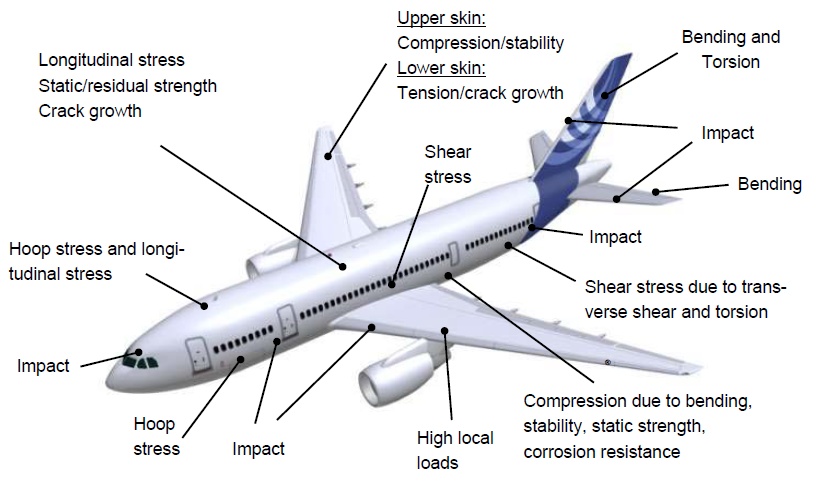
\includegraphics[width=125mm]{2/Fotos/Aircraft_Sress.png}
    \caption{Problemas asociados a las estructuras de una aeronave} % \cite{stress}
    \label{stress}
\end{figure}

En aeronáutica, la inmensa mayoría de partes se diseñan a fatiga. Esto quiere decir que, para un número determinado de ciclos y con un espectro determinado de cargas, la pieza o estructura no compromete la integridad global de la aeronave.

Dentro del diseño a fatiga hay otras dos tendencias, el diseño a vida segura o a tolerancia al daño. En las estructuras diseñadas bajo el criterio de vida segura granizan que, mientras no se supere el espectro de carga, la integridad estructural no peligra. En cambio, el diseño de tolerancia al daño tiene en cuenta que en el propio proceso de fabricación se generan grietas en el material y asume que estas grietas van a crecer, por lo que toma medidas para asegurar que no se produzcan fallos catastróficos \cite{criterios}. 

\vspace*{10pt}
\begin{figure}[ht]
    \centering
    \begin{tikzpicture}[edge from parent fork down]
        \tikzstyle{every node}=[rectangle, draw=black, thick, text width=7em, text centered, rounded corners,minimum height=5mm, minimum width=20mm,minimum height=10mm]
        \tikzstyle{edge from parent}=[black,-,thick,draw]
        \footnotesize
        \node {Diseño a Fatiga}
        child {node [xshift=-7.5mm] {Vida segura}}
        child {node [xshift=7.5mm] {Tolerancia al daño}
        child {node [xshift=-7.5mm] {Fallo seguro}
        child {node [xshift=-7.5mm] {Bloqueo de grieta}}
        child {node [xshift=7.5mm] {Camino de carga múltiple}}}
        child {node [xshift=7.5mm] {Crecimiento lento}}
        };
    \end{tikzpicture}
    \caption{Criterios de diseño \cite{criterios}}
    \label{des_cri}
\end{figure}
\vspace*{10pt}

Usando las Figuras \ref{stress} y \ref{des_cri} se puede tener una idea general de la estructura bajo estudio y responder a la primera pregunta. El siguiente paso será diferenciar entre los distintos daños que pueden sufrir estas estructuras.

%------------%

\subsection{Daños en estructuras aeronáuticas}

% En una estructura aeronáutica, se puede definir un daño como los cambios en el material y/o en las propiedades geométricas de un sistema estructural, incluyendo cambios en las condiciones de contorno y conectividad del mismo, que pueden afectar de manera adversa al funcionamiento presente y futuro del sistema \cite{dam}.\\

% Como este trabajo se va a centrar en daños sobre estructuras fabricadas en material compuesto, 
 
% De forma general, se pueden organizar los daños que sufren las estructuras aeronáuticas dentro de las siguientes categorías \cite{Jaime_Tesis}:

% \begin{itemize}
%     \item[\textbullet] \textbf{Daño accidental}: daño fortuiro y no predecible que se produce en la estructura. Por ejemplo, un impacto de pájaro.
%     \item[\textbullet] \textbf{Daño por fatiga}: este es un tipo de daño predecible, derivado de la acción de las cargas cíclicas en la misma. Un ejemplo son las grietas que aparecen en el perímetro de agujeros.
%     \item[\textbullet] \textbf{Daño ambiental}: este tipo no es predecible, se produce en la estructura por acción del medio ambiente en el que opera la estructura. Uno de los ejemplos es la corrosión.
%     \item[\textbullet] \textbf{Daño operacional}: al igual que los accidentales, es un daño no predecible y fortuito que se produce en la estructura derivado de la operación de la misma. Un caso común es una sobrecarga en la maniobra de aterrizaje.
% \end{itemize}

% Como ya se ha comentado anteriormente, este trabajo se va a centrar en estructuras fabricadas en Material Compuesto. Los modos de fallo que se producen en este tipo de material son diferentes a los que ocurren en las estructuras metálicas \cite{dam_comp} y a continuación se presenta un breve resumen de estos tipos característicos de daños \cite{comp}.

% \begin{itemize}
%     \item[\textbullet] \textbf{Daño por tracción}: este fallo es producido por varios mecanismos de daño que ocurren secuencialmente. Usando como referencia la Figura \ref{traccion} se tiene un laminado [0,90,0] con una carga longitudinal aplicada en la orientación 0º. Cuando comienza un ciclo de carga, primero se rompe la lámina orientada a 90º ya que la resina es la que soporta los mayores esfuerzos. Cuando aumenta la carga, comienzan a aparecer delaminaciones entre las pieles debido a tensiones generadas por efectos tridimensionales. Si sigue aumentando la carga, se llega a rotura final de la fibra.
%     \begin{figure}[ht]
%         \centering
%         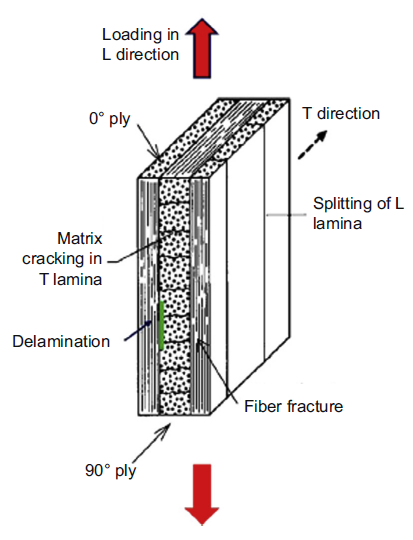
\includegraphics[width=50mm]{2/Fotos/traccion.png}%
%         \caption{Tracción axial}
%         \label{traccion}
%     \end{figure}
    
%     \item[\textbullet] \textbf{Daño en compresión}: cuando se somete a estructura a compresión axial, el compuesto falla por pandeo. En una escala local, el material falla por el mecanismo de micropandeo. Al estar las fibras en una matriz flexible, al aplicar la carga las fibras se empiezan a ondular, como se ve en la Figura \ref{pandeo-a}. Conforme aumenta la carga la ondulación aumenta hasta que se produce el fallo en forma de \textit{kink bands}, en las Figuras \ref{pandeo-b} y \ref{pandeo-c} se puede apreciar el fenómeno.
%     \begin{figure}[ht]
%         \centering
%         \subfloat[Ondulación de las fibras]{%
%           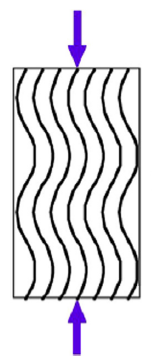
\includegraphics[width=22.5mm]{2/Fotos/pandeo-a.png}%
%           \label{pandeo-a}%
%         }\qquad
%         \subfloat[Falla local de banda]{%
%           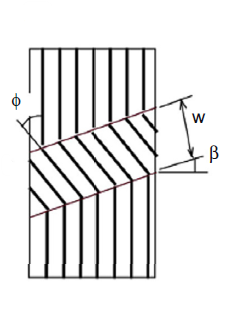
\includegraphics[width=35mm]{2/Fotos/pandeo-b.png}%
%           \label{pandeo-b}%
%         }
%         \subfloat[Micrografía de falla local de banda]{%
%           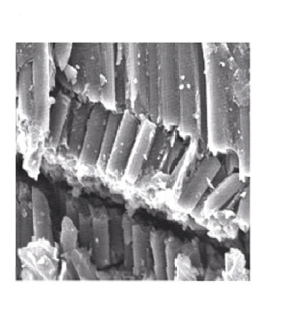
\includegraphics[width=45mm]{2/Fotos/pandeo-c.png}%
%           \label{pandeo-c}%
%         }
%         \caption{Daño por compresión en compuestos por micropandeo}
%     \end{figure}
    
%     \item[\textbullet] \textbf{Daños en agujeros de unión}: cuando se quiere unir una pieza metálica con otra de compuesto, un método ampliamente usado es la unión con elementos mecánicos, lo que lleva a realizar agujeros y tiene una gran penalización en la rigidez y fatiga. Se pueden dar causados por tracción, Figura \ref{agujero-a}, o por compresión, Figura \ref{agujero-b}.
%     \begin{figure}[ht]
%         \centering
%         \subfloat[Fallos por tracción]{%
%           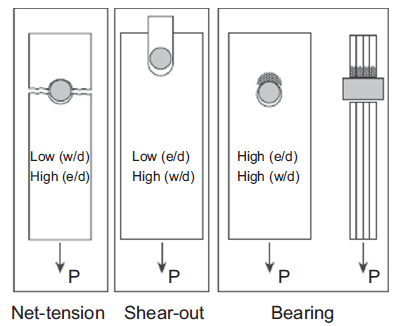
\includegraphics[width=65mm]{2/Fotos/agujero-a.png}%
%           \label{agujero-a}%
%         }\qquad
%         \subfloat[Fallos por compresión]{%
%           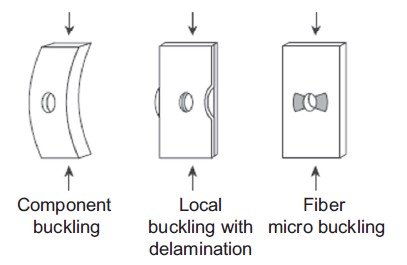
\includegraphics[width=75mm]{2/Fotos/agujero-b.png}%
%           \label{agujero-b}%
%         }
%         \caption{Distintos daños en agujeros de unión}
%     \end{figure}
    
%     \item[\textbullet] \textbf{Daño por impacto}: este tipo de daño no es importante en estructuras metálicas, sin embargo, un impacto de baja velocidad puede generar daños importantes y sin dejar ninguna marca en la superficie. Cuando el impacto es de baja energía puede generar delaminaciones y si tiene la energía suficiente producirá desconchado en la superficie opuesta al impacto. Se puede ver el esquema de las etapas que sufre un laminado unidireccional bajo una carga cíclica en la Figura \ref{delaminacion}. 
%     \begin{figure}[ht]
%         \centering
%         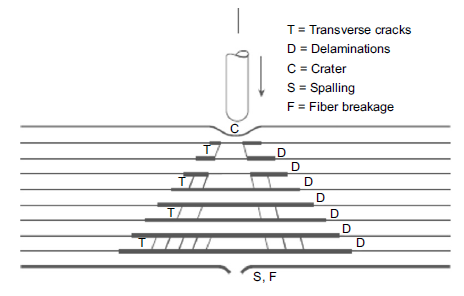
\includegraphics[width=125mm]{2/Fotos/delamination.png}%
%         \caption{Consecuencias de un impacto en material compuesto}
%         \label{delaminacion}
%     \end{figure}
    
%     \item[\textbullet] \textbf{Daño por fatiga}: la fatiga en compuestos es más complicada que en materiales metálicos. En la Figura \ref{fatiga}. La evolución del daño por estas fases depende del nivel de carga en el ciclo de fatiga.
%     \begin{figure}[ht]
%         \centering
%         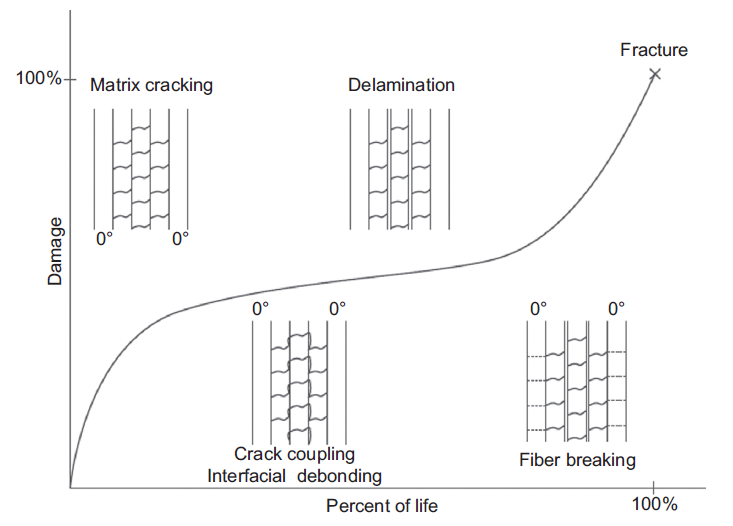
\includegraphics[width=125mm]{2/Fotos/fatiga.png}%
%         \caption{Etapas de crecimiento de daño en fatiga}
%         \label{fatiga}
%     \end{figure}
    
%     \item[\textbullet] \textbf{Daño en estructuras sandwich}: los paneles sandwich de polímero reforzado con fibra de carbono (CFRP)son mucho más sucreptibles al daño por impacto que los fabricados con polímero reforzado con fibra de vidrio (GFRP), y el tipo de daño predominante en cada uno de ellos es diferente. La rotura de fibra en CFRP sandwich y el aplastamiento del núcleo en los paneles fabricados con GFRP. En la Figura \ref{sandwich} se pueden ver diversos daños que estos paneles pueden sufrir.
%     \begin{figure}[ht]
%         \centering
%         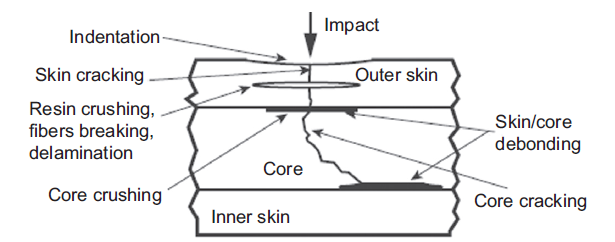
\includegraphics[width=125mm]{2/Fotos/sanwich.png}%
%         \caption{Daños típicos en paneles sandwich}
%         \label{sandwich}
%     \end{figure}
    
%     \item[\textbullet] \textbf{Daño en uniones adhesivas}: la unión adhesiva es ventajosa frente la mecánica, ya que el hacer agujeros presenta muchos problemas. Sin embargo, la fiabilidad de las uniones adhesivas no siempre se puede garantizar. La delaminación en uniones adhesivas de compuestos es el daño más frecuente, lo que reduce la rigidez de la estructura y con ello la capacidad de carga de la estructura.
% \end{itemize}

% Estos daños se pueden producir de forma conjunta y, de hecho, la inmensa mayoría de ellos aparecen en fuselajes o elementos de pared delgada.\\

% Una vez que se tiene la lista de posibles daños que pueden afectar a una estructura se necesita encontrar cuál de todos los parámetros medibles en esta estructura se ve afectado por la presencia del daño, la DSF.

% A su vez, hay que tener en cuenta como el daño modifica la DSF a medida que crece. Esta relación se llama Firma de Daño (FdD). Dicha firma puede ser algún valor relacionado con la medida o señal que se obtiene de la DSF.

% Una vez definidas la DSF y la FdD apropiadas para la estructura que se esté estudiando, se puede pasar a la elección de la tecnología SHM a aplicar.\\

% \textbf{METER LA TABLA DE JAIME CON LAS CARACTERÍSTICAS SENSITIVAS QUE SE VEN AFECTADAS POR CADA DAÑO?}


% \subsection{Tecnologías SHM}

% Una de las formas de clasificar las diferentes técnicas de SHM consiste en evaluar la física que hay detrás de ellas. Para un mejor entendimiento se ha dibujado un mapa conceptual que relaciona las tecnologías con los sensores.

% \vspace*{10pt}
% \begin{figure}[ht]
%     \centering
%     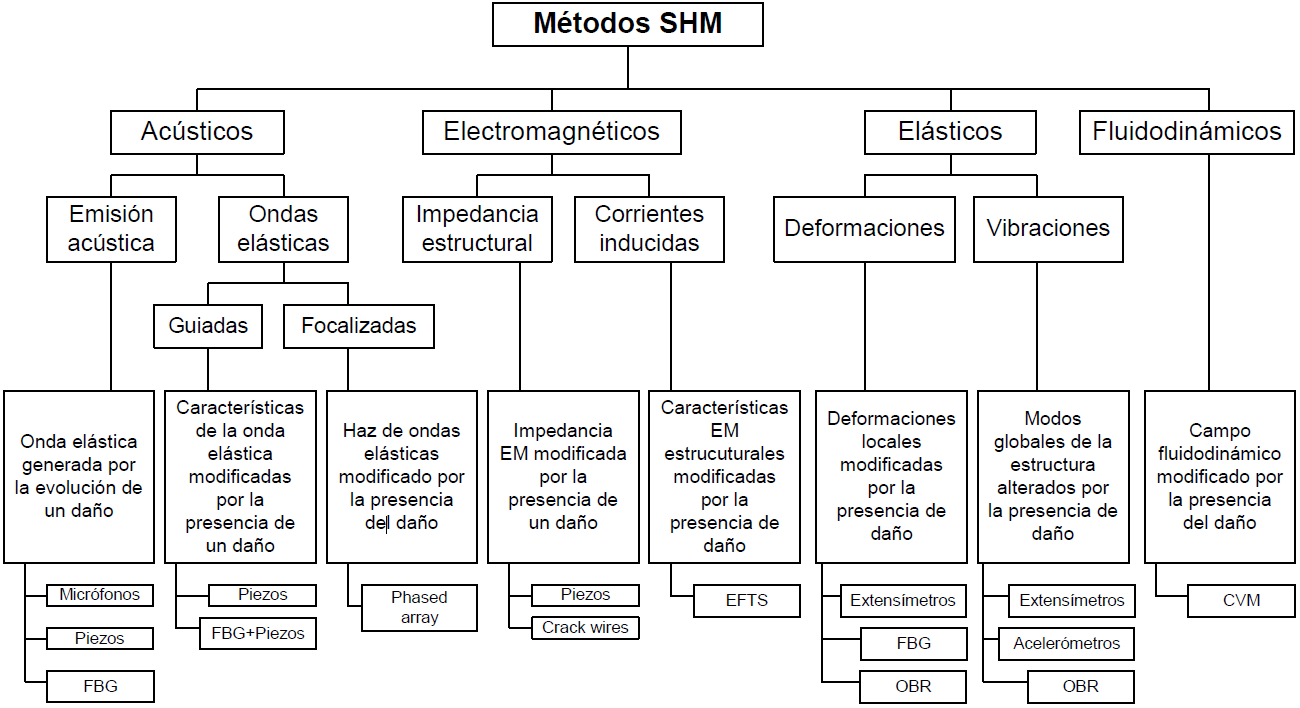
\includegraphics[width=\textwidth]{2/Fotos/shm_tec.png}
%     \caption{Tecnología SHM \cite{shm_tec}}
%     \label{}
% \end{figure}
% \vspace*{10pt}

% Una vez sabiendo los sensores y tecnologías SHM disponibles junto a los daños típicos, se puede construir una tabla para hacer más sencilla la elección de una tecnología para un determinado daño y DSF \cite{Jaime_Tesis}.

% \begin{table}[H]
%     \centering
%     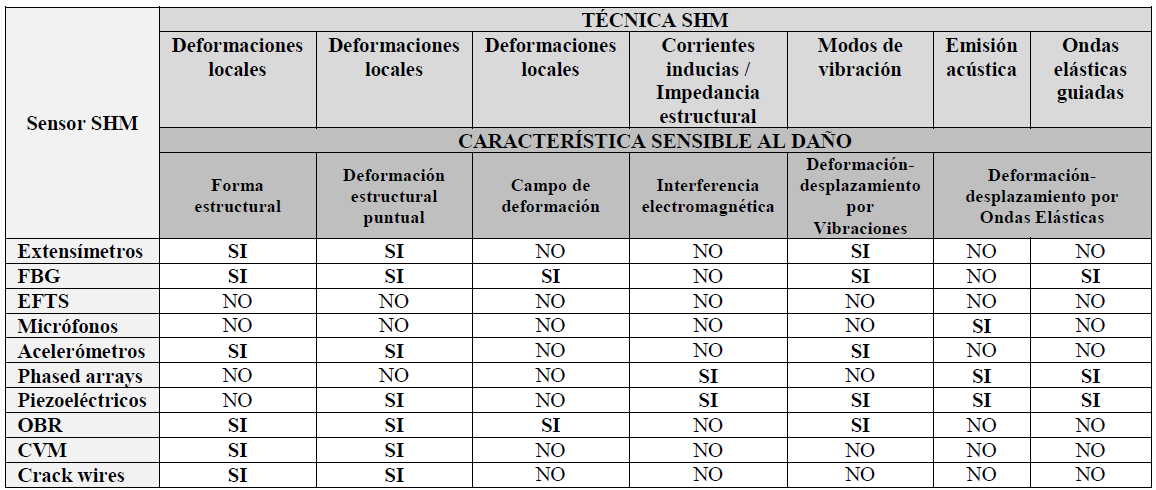
\includegraphics[width=\textwidth]{2/Fotos/DSF_tec.png}
%     \caption{Relación entre sensores y técnicas de SHM con DSF \cite{Jaime_Tesis}}
%     \label{dsf_tec}
% \end{table}



\clearpage

% -- -- %


\section{Inteligencia Artificial aplicada a SHM}  %{Machine Learning SHM}

2-3 pags

\begin{enumerate}
    \item Explicar que es la inteligencia artificial y lo tipos que hay
    \item Diferencias que hay entre Machine learning y Deep learning y por qué decidimos que el Deep Learning es mejor para nuestro objetivo
    \item Comentar las distintas redes neuronales dentro de DL y argumentos para elegir las Recurrent Neural Networks - RNN
    \item Ejemplos de IA aplicada en SHM
\end{enumerate}

\subsection{Representación gráfica del funcionamiento de una Red Neuronal}
\label{sec:funcionamiento_DL}

Aunque el campo del DL lleva unos años en auge, para la mayoría de usuarios sigue siendo una simple herramienta, es desconocido cómo funciona y mucho menos se tiene una representación gráfica de qué hace y cómo llega a los resultados.

Dado que este trabajo se va a centrar en tecnología de DL, es conveniente hacer una breve explicación de cómo una NN es capaz de clasificar diferentes grupos de datos. Para ello, esta explicación se ha basado en el gran trabajo realizado por el equipo de \textit{TensorFlow - playground} \cite{TensorFlow_playground}. Un entorno perfecto para la visualización del comportamiento de los diferentes parámetros que componen una Red Neuronal.\\

Lo primero de todo es saber la forma de los argumentos de entrada que, como para casi todo algoritmo, sus \textit{inputs} son números. Dependiendo del problema que se busque resolver estos datos tendrán una forma u otra, más complejos o más simples, pero en esta introducción se va a utilizar un dataset de 2 dimensiones ($x_1,x_2$) y dos clases diferentes (azul y naranja).

Los datos que se van a intentar clasificar están representados en la Figura \ref{datos}

\begin{figure}[h!]
    \centering
    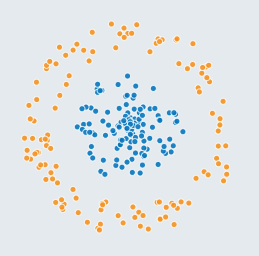
\includegraphics[width=60mm, angle=0]{2/Fotos/datos.png}
    \captionsetup{justification=centering,margin=1.25cm}
    \caption{Representación de las dos clases diferentes en dos colores}
    \label{datos}
\end{figure}

Una vez se conocen los dos grupos que se busca clasificar se va a comenzar la descripción de los elementos que componen una NN y como interactúan entre ellos. Estos elementos son:

\begin{itemize}
    \item[\tiny{\textbullet}] \textbf{Neurona}
    
    Es la unidad básica de procesamiento que compone una Red Neuronal. Estas neuronas tienen conexiones a través de las que reciben los valores de entrada y realizan una suma ponderada con ellos. Cada una de las entradas es multiplicada por un valor, llamado peso, que definirá a cual de los valores de entrada se le da más importancia. A este cálculo se le añadirá un sesgo o \textit{bias}, dicho de otro modo, se le sumará un escalar.
    
    Si se observa detenidamente la Figura \ref{perceptron} (primera neurona llamada \textit{perceptron}) se puede ver que, matemáticamente, una neurona es equivalente a una regresión lineal ($w_1 \cdot x_1 + w_2 \cdot x_2 + b = 0$).
    
    \begin{figure}[H]
        \centering
        \begin{tikzpicture}[
            init/.style={
              draw,
              circle,
              inner sep=2pt,
              font=\Huge,
              join = by -latex
            },
            squa/.style={
              draw,
              inner sep=2pt,
              font=\Large,
              join = by -latex
            },
            start chain=2,node distance=13mm
            ]
            \node[on chain=2] 
              (x2) {$x_2$};
            \node[on chain=2,join=by o-latex] 
              {$w_2$};
            \node[on chain=2,init] (sigma) 
              {$\displaystyle\Sigma$};
            % \node[on chain=2,squa,label=above:{\parbox{2cm}{\centering Activate \\ function}}]   
            %   {$f$};
            \node[on chain=2,label=above:Output,join=by -latex] 
              {$y$};
            \begin{scope}[start chain=1]
            \node[on chain=1] at (0,1.5cm) 
              (x1) {$x_1$};
            \node[on chain=1,join=by o-latex] 
              (w1) {$w_1$};
            \end{scope}
            \begin{scope}[start chain=3]
            \node[on chain=3] at (0,-1.5cm) 
              (x3) {$x_3$};
            \node[on chain=3,label=below:Weights,join=by o-latex] 
              (w3) {$w_3$};
            \end{scope}
            \node[label=above:\parbox{2cm}{\centering Bias \\ $b$}] at (sigma|-w1) (b) {};
            
            \draw[-latex] (w1) -- (sigma);
            \draw[-latex] (w3) -- (sigma);
            \draw[o-latex] (b) -- (sigma);
            
            \draw[decorate,decoration={brace,mirror}] (x1.north west) -- node[left=10pt] {Inputs} (x3.south west);
        \end{tikzpicture}
        \captionsetup{justification=centering,margin=1.25cm}
        \caption{Representación del \textit{perceptron}}
        \label{perceptron}
    \end{figure}
    
    En una regresión lineal bidimensional, ajustando los pesos ($w_1,w_2$) se modifica la recta que separa el plano ($x_1,x_2$) en dos regiones. En el ejemplo que se está resolviendo, por muy bien que se ajusten estos pesos, con una neurona solo se puede llegar a separar el plano en dos regiones, como se ve en la Figura \ref{neurona}.
    
    \begin{figure}[h!]
        \centering
        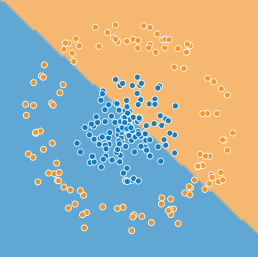
\includegraphics[width=60mm, angle=0]{2/Fotos/neurona.png}
        \captionsetup{justification=centering,margin=1.25cm}
        \caption{Clasificación de datos con una sola neurona}
        \label{neurona}
    \end{figure}
    
    Para definir que región del plano es asignada a la clase azul o naranja se utiliza la siguiente expresión:
    
    \begin{equation}
        w_1 \cdot x_1 + w_2 \cdot x_2 + b = y \hspace*{5pt}
        \begin{cases}
            y \geq 0, & naranja\\
            y < 0, & azul%\text{otherwise}
        \end{cases}
        \label{eq:percepron}
    \end{equation}

    Por lo tanto, la neurona se puede sintetizar un una función. Como una neurona no consigue separar las dos regiones de puntos de forma efectiva, hace que sea necesario dar un paso más.
    
    
    %https://tex.stackexchange.com/questions/132444/diagram-of-an-artificial-neural-network
    
    \item[\tiny{\textbullet}] \textbf{Capas}
    
    Para modelizar conocimiento complejo no es suficiente con utilizar una única neurona, es necesario concatenar varias de ellas. Una forma de colocar las neuronas sería una debajo de otra en forma de columna, lo que se define como, en la misma capa.
    
    \begin{figure}[H]
        \centering
        \tikzset{%
          every neuron/.style={
            circle,
            draw,
            minimum size=1cm
          },
          neuron missing/.style={
            draw=none, 
            scale=4,
            text height=0.333cm,
            execute at begin node=\color{black}$\vdots$
          },
        }
        \begin{tikzpicture}[x=1.5cm, y=1.5cm, >=stealth]
            \foreach \m/\l [count=\y] in {1,2,3,missing,4}
              \node [every neuron/.try, neuron \m/.try] (input-\m) at (0,2.5-\y) {};
            \foreach \m [count=\y] in {1,missing,2}
              \node [every neuron/.try, neuron \m/.try ] (hidden-\m) at (2,2-\y*1.25) {};
            \foreach \m [count=\y] in {1,missing,2}
              \node [every neuron/.try, neuron \m/.try ] (output-\m) at (4,1.5-\y) {};
            \foreach \l [count=\i] in {1,2,3,n}
              \draw [<-] (input-\i) -- ++(-1,0)
                node [above, midway] {$I_\l$};
            \foreach \l [count=\i] in {1,n}
              \node [above] at (hidden-\i.north) {$H_\l$};
            \foreach \l [count=\i] in {1,n}
              \draw [-latex] (output-\i) -- ++(1,0)
                node [above, midway] {$O_\l$};
            \foreach \i in {1,...,4}
              \foreach \j in {1,...,2}
                \draw [-latex] (input-\i) -- (hidden-\j);
            \foreach \i in {1,...,2}
              \foreach \j in {1,...,2}
                \draw [-latex] (hidden-\i) -- (output-\j);
            \foreach \l [count=\x from 0] in {Input, Hidden, Ouput}
              \node [align=center, above] at (\x*2,2) {\l \\ layer};
        \end{tikzpicture}
        \captionsetup{justification=centering,margin=1.25cm}
        \caption{Representación de las capas de una red}
        \label{capas}
    \end{figure}
    
    Como se representa en la Figura \ref{capas}, las capas se pueden concatenar de manera secuencial, una detrás de otra y dependiendo de dónde estén colocadas tendrán un nombre u otro. La capa que recibe primero los argumentos de entrada se llama \textit{Input layer}, la que calcula el argumento de salida se llama \textit{Output layer} y todas las capas que estén entre estas dos, se llamarán \textit{Hidden layers}. 
    
    La concatenación secuencial de las capas hace que la red sea capaz de aprender conocimiento jerarquizado y es lo que da nombre al Deep Learning (Aprendizaje Profundo). Dicho de otro modo, si a la red se le introduce una imagen de un coche, es capaz de aprender que un coche no es un objeto único, una capa sintetiza lo que es una rueda, la siguiente lo que es una puerta y las últimas capas son capaces de juntar toda esa información para construir la idea de coche como un conjunto de objetos.
    
    Las neuronas dentro de la misma capa lo que permiten es diversificar el conocimiento. Cada neurona se especializa en una parte de la información ajustando los pesos para dar más importancia a un canal de entrada u otro.
    
    Juntando lo explicado anteriormente se entiende mejor este concepto de aprendizaje. Una red parte de una cantidad grande de datos, los píxeles de una imagen, por ejemplo. La capa de entrada será la que primero reciba la información, por ello necesitará muchas neuronas para procesarla y extraer de ella qué zonas de la imagen son más importantes. A medida que se va avanzando, cada una de las capas tiene que desglosar cada vez más la información sintetizada que le ha llegado de la capa anterior, por lo que necesitará menos neuronas, su nivel de abstracción de conocimiento aumenta.
    
    \begin{figure}[h!]
        \centering
        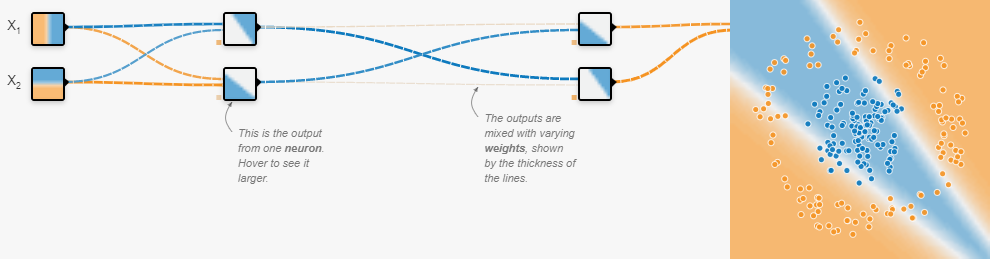
\includegraphics[width=135mm, angle=0]{2/Fotos/capas.png}
        \captionsetup{justification=centering,margin=1.25cm}
        \caption{Red con dos \textit{Hidden layers} y dos neuronas en cada capa}
        \label{aplicacion_capas}
    \end{figure}
    
    La aplicación de lo explicado anteriormente se representa en la Figura \ref{aplicacion_capas}. Se puede observar en la caja que representa cada neurona que, en esencia, todas hacen una regresión lineal y que no pueden crear una frontera circular para separar el espacio. Esto se debe a que la operación matemática de concatenación de regresiones lineales termina colapsando en una regresión lineal, no puede dibujar curvas. Para conseguirlo, es necesario añadir un elemento más. 
    

    \item[\tiny{\textbullet}] \textbf{Función de activación}
    
    La necesidad de aplicar una distorsión no lineal a la salida de las neuronas convierte en indispensables a las funciones de activación. Con ellas se podrá encadenar de forma efectiva la computación de varias neuronas.
    
    \begin{figure}[h!]
        \centering
        \begin{tikzpicture}[
            init/.style={
              draw,
              circle,
              inner sep=2pt,
              font=\Huge,
              join = by -latex
            },
            squa/.style={
              draw,
              inner sep=2pt,
              font=\Large,
              join = by -latex
            },
            start chain=2,node distance=13mm
            ]
            \node[on chain=2] 
              (x2) {$x_2$};
            \node[on chain=2,join=by o-latex] 
              {$w_2$};
            \node[on chain=2,init] (sigma) 
              {$\displaystyle\Sigma$};
            \node[on chain=2,squa,label=above:{\parbox{2cm}{\centering Activate \\ function}}]   
              (f) {$f$};
            \node[on chain=2,label=above:Output] 
              (y) {$y$};
            \begin{scope}[start chain=1]
            \node[on chain=1] at (0,1.5cm) 
              (x1) {$x_1$};
            \node[on chain=1,join=by o-latex] 
              (w1) {$w_1$};
            \end{scope}
            \begin{scope}[start chain=3]
            \node[on chain=3] at (0,-1.5cm) 
              (x3) {$x_3$};
            \node[on chain=3,label=below:Weights,join=by o-latex] 
              (w3) {$w_3$};
            \end{scope}
            \node[label=above:\parbox{2cm}{\centering Bias \\ $b$}] at (sigma|-w1) (b) {};
            
            \draw[-latex] (w1) -- (sigma);
            \draw[-latex] (w3) -- (sigma);
            \draw[o-latex] (b) -- (sigma);
            
            \draw[decorate,decoration={brace,mirror}] (x1.north west) -- node[left=10pt] {Inputs} (x3.south west);
            \draw[decorate,decoration={coil,aspect=0}] (f.east) -- (y.west);
        \end{tikzpicture}
        \captionsetup{justification=centering,margin=1.25cm}
        \caption{Efecto de la función de activación sobre el output de una neurona}
        \label{perceptron_act}
    \end{figure}
    
    En cierto modo ya se estaba usando una función de activación antes de nombrarlas. En la Ecuación \ref{eq:percepron} se había usado la función escalón para separar las dos regiones del plano, pero esta función no provoca no linealidades y no es muy efectiva cuando se requieren fronteras complejas. 
    
    \vspace*{5pt}
    \begin{figure}[h!]
        \centering
        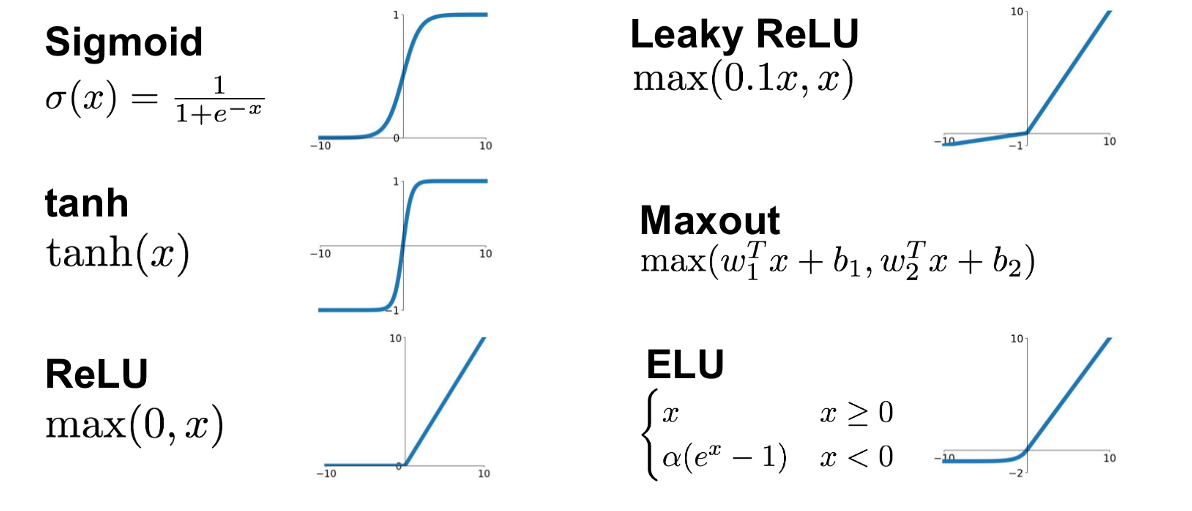
\includegraphics[width=135mm, angle=0]{2/Fotos/activation_functions.png}
        \captionsetup{justification=centering,margin=1.25cm}
        \caption{Funciones de activación más populares}
        \label{activation_functions}
    \end{figure}
    
    Las funciones de activación más conocidas están representadas en la Figura \ref{activation_functions}. Su función principal es hacer que los valores muy grandes o muy pequeños se saturen a determinado valor, dependiendo de la función elegida. 
    
    Para ver el efecto de distorsión geométrica que tienen estas funciones sobre el \textit{output} de las neuronas se usa de ejemplo la Figura \ref{single_sigmoid}. La nueva función de salida se convierte en una superficie, continua y derivable, que para cada \textit{input} ($x_1,x_2$) le corresponde una altura $y$ entre 0 y 1. 
    
    Tal y como se ha hecho anteriormente, se selecciona un valor umbral de $y$ a partir del cual se clasificarán los puntos como azules o naranjas. En la Figura \ref{single_sigmoid} este valor umbral se representa como un plano a una altura de $0.5$, por lo tanto, los puntos ($x_1,x_2$) que tras ser evaluados en la neurona saquen un valor de $y$ inferior a $0.5$ se clasificarán como \textit{naranjas} y los que den un valor superior o igual a $0.5$ se clasificarán como \textit{azules}. Esto recuerda a la Figura \ref{neurona}.

    \vspace*{5pt}
    \begin{figure}[h!]
        \centering
            \subfloat[Vista en perspectiva]{%
              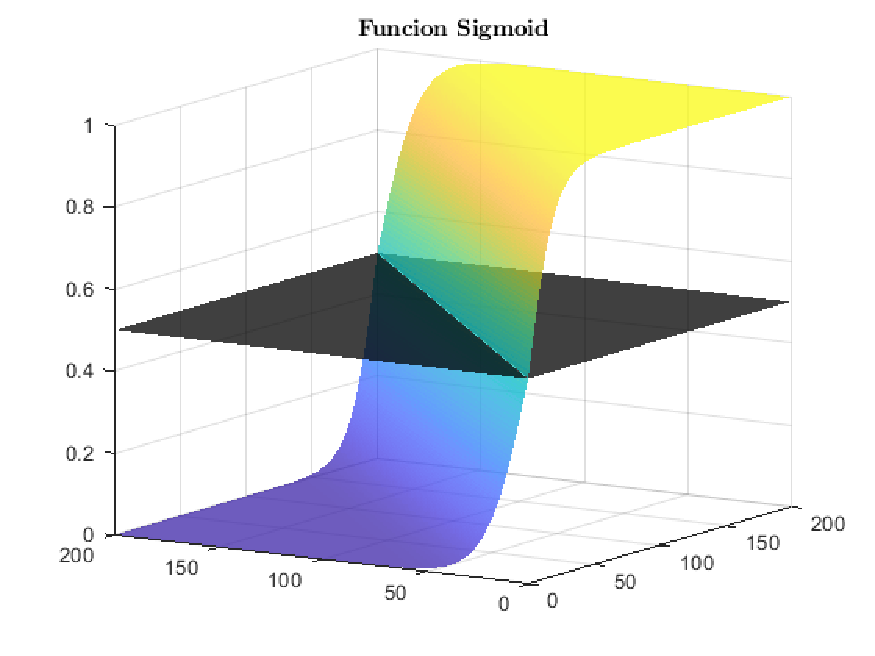
\includegraphics[width=70mm]{2/Fotos/single_sigmoid.pdf}%
              \label{}%
            }\qquad
            \subfloat[Vista perpendicular al plano de valor \textit{z = 0.5}]{%
              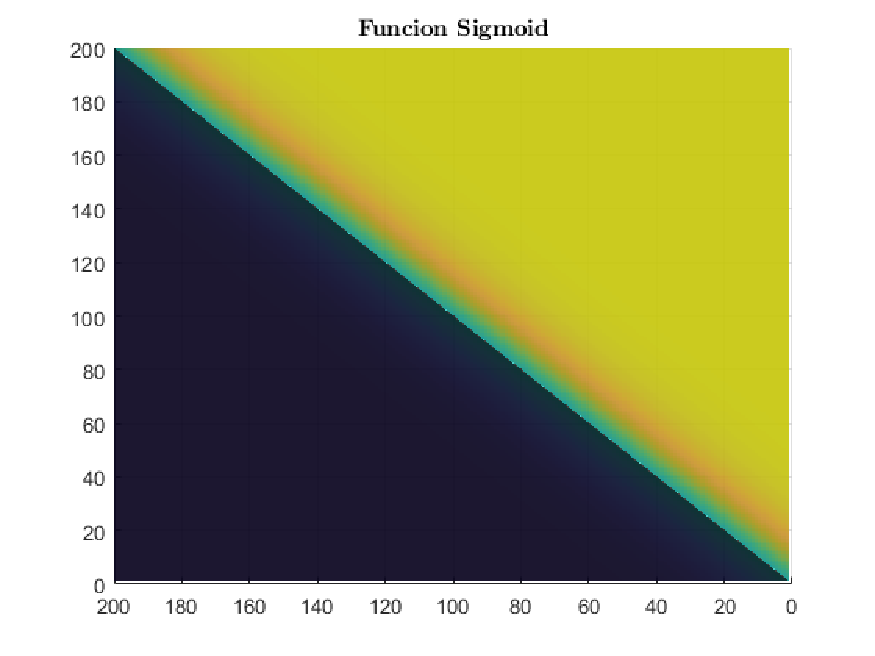
\includegraphics[width=70mm]{2/Fotos/single_sigmoid_top.pdf}%
              \label{}%
            }
        \caption{Combinación de funciones de activación}
        \label{single_sigmoid}
    \end{figure}
    
    Ahora ya se puede utilizar una \textit{hidden layer} con varias neuronas de forma efectiva. La combinación de varias neuronas hace que se sumen superficies (funciones) como la representada en la Figura \ref{single_sigmoid}, pero con diferentes orientaciones, generando superficies más complejas, Figura \ref{combinacion_sigmoid}. Igual que antes, los puntos ($x_1,x_2$) que tras ser evaluados tienen un $y$ mayor o igual a $0.5$ pertenecerán a la clase azul y los menores a la naranja.
    
    \vspace*{5pt}
    \begin{figure}[h!]
        \centering
            \subfloat[Vista en perspectiva]{%
              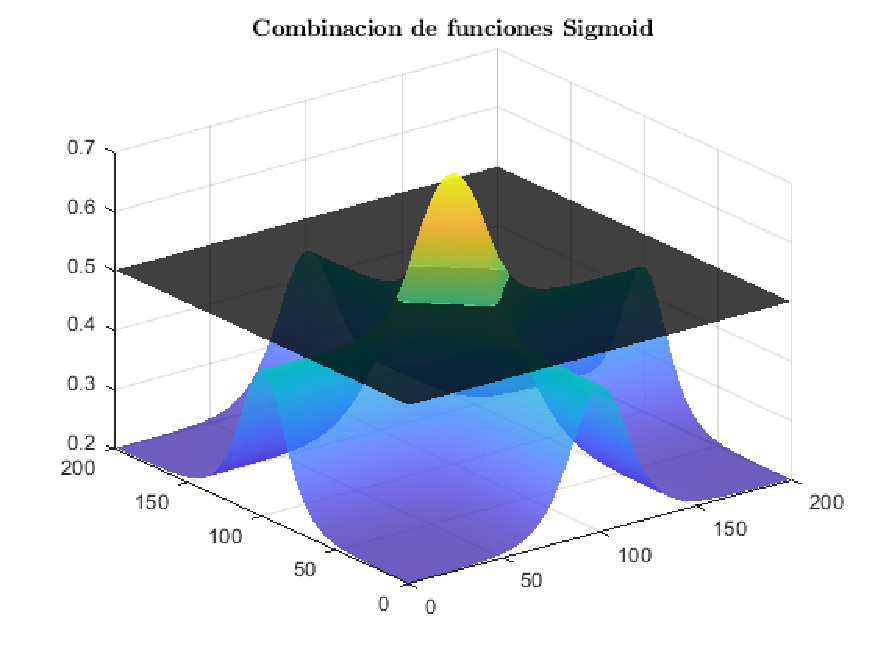
\includegraphics[width=70mm]{2/Fotos/combinacion_softmax.pdf}%
              \label{}%
            }\qquad
            \subfloat[Vista perpendicular al plano de valor \textit{z = 0.5}]{%
              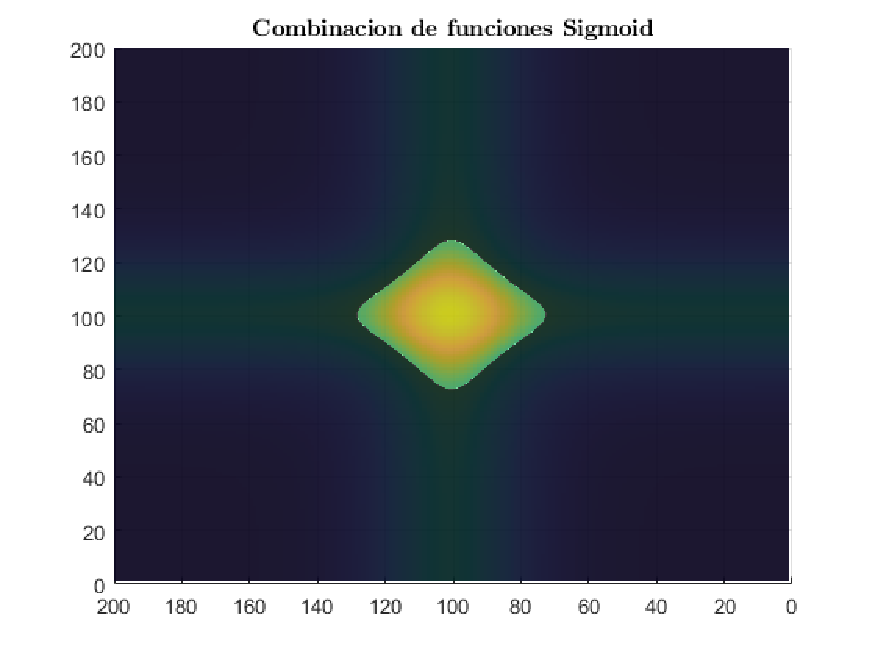
\includegraphics[width=70mm]{2/Fotos/combinacion_softmax_top.pdf}%
              \label{}%
            }
        \caption{Combinación de funciones de activación}
        \label{combinacion_sigmoid}
    \end{figure}
    
    Finalmente se puede ver en la Figura \ref{clasificacion_activacion} la aplicación de todo lo explicado. Gracias a las funciones de activación se consiguen las no linealidades necesarias para generar la superficie que separe exitosamente las dos clases de datos diferentes. 
    
    \vspace*{5pt}
    \begin{figure}[h!]
        \centering
        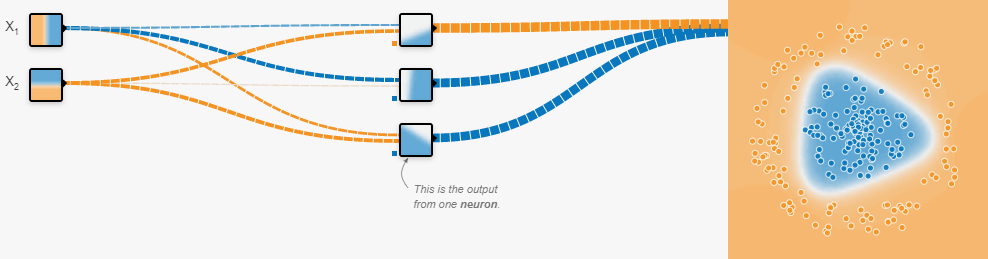
\includegraphics[width=135mm, angle=0]{2/Fotos/clasificacion_activacion.png}
        \captionsetup{justification=centering,margin=1.25cm}
        \caption{Resultado final de la clasificación}
        \label{clasificacion_activacion}
    \end{figure}
    
    Las neuronas de la Figura \ref{clasificacion_activacion} están unidas mediante unas líneas discontinuas de diferente color y grosor. Esto representa qué pesos son mayores y que zona perturban más. Los pesos son los elementos que ajustan las funciones de activación para conseguir la superficie final que mejor realice la clasificación. Pero, ¿cómo se realiza el ajuste de los pesos?
    
    \item[\tiny{\textbullet}] \textbf{Entrenamiento}
    
    Se llama entrenamiento al proceso de aprendizaje automático que utilizan las redes neuronales para ajustar sus parámetros internos. El algoritmo que hizo posible que la optimización de parámetros en DL fuera eficiente se llama \textit{backpropagation} y es el responsable del final del \textit{Invierno de la Inteligencia Artificial}
    
    Para llevar a cabo el proceso de optimización es necesario calcular las derivadas parciales de cada uno de los parámetros de la red con respecto a la función de error. Una vez se consigan las derivadas, se utilizará el algoritmo de descenso del gradiente para variar los parámetros y minimizar la función de error.
    
    La función de error ($E$) puede ser, por ejemplo, la suma de las distancias de cada punto a la frontera de su clase. Volviendo a la Figura \ref{neurona}, los puntos azules que se encuentran en la región naranja aumentarán mucho el valor de la función de error, mientras que los que están en la región azul no aumentarán casi su valor. La variación de la función de error respecto a un pequeño cambio los parámetros se representa matemáticamente como el gradiente gradiente: $\frac{\partial E}{\partial w}$.
    
    Como se ve en la Figura \ref{fig:prop_error}, el peso asociado a una de las primeras conexiones afecta a prácticamente todas las conexiones posteriores y por lo tanto, también influirán en su gradiente. Esto hace que el aprendizaje de este primer peso sea especialmente complicado y convierte en esencial la utilización del \textit{backpropagation} para el proceso de optimización.
    
    \begin{figure}[h!]
        \centering
        \begin{tikzpicture}
        	\tikzstyle{place}=[circle, draw=black, minimum size = 8mm]
        	% Input
        	\foreach \x in {1,...,2}
        		\draw node at (0, -1.25-\x*1.25) [place] (first_\x) {$x_\x$};
        	% Hidden 1
         	\foreach \x in {1,...,4}
         		\node at (2, -\x*1.25) [place] (second_\x){};%{$n_{1,\x}$};
        	% Hidden 2
        	\foreach \x in {1,...,4}
        		\node at (4, -\x*1.25) [place] (third_\x){};%{$n_{2,\x}$};
        	% Hidden 3
         	\foreach \x in {1,...,4}
         		\node at (6, -\x*1.25) [place] (fourth_\x){};%{$n_{3,\x}$};
        	% Output
        	\foreach \x in {1,...,1}
            		\node at (8, -\x*3.125) [place] (fifth_\x){$y$};
        	%---------------------%
        	% Input -> Hidden 1
        	\foreach \i in {1,...,2}
        		\foreach \j in {1,...,4}
        			\draw [-latex] (first_\i) to (second_\j);
        	% Hidden 1 -> Hidden 2
        	\foreach \i in {1,...,4}
        		\foreach \j in {1,...,4}
        			\draw [-latex] (second_\i) to (third_\j);
        	% Hidden 1 -> Hidden 3
        	\foreach \i in {1,...,4}
        		\foreach \j in {1,...,4}
        			\draw [-latex] (third_\i) to (fourth_\j);
        	% Hidden 3 -> Output
        	\foreach \i in {1,...,4}
    		\foreach \j in {1,...,1}
        			\draw [-latex] (fourth_\i) to (fifth_\j);
            %---------------------%
            \foreach \k in {1,...,3}{
                % Input -> Hidden 1
                \draw[red] [-latex] (first_1) to (second_1);
                % Hidden 1 -> Hidden 2
                \foreach \i in {1,...,1}
                	\foreach \j in {1,...,4}
                		\draw[red] [-latex] (second_\i) to (third_\j);
                % Hidden 2 -> Hidden 3
                \foreach \i in {1,...,4}
                	\foreach \j in {1,...,4}
                		\draw[red] [-latex] (third_\i) to (fourth_\j);
                % Hidden 3 -> Output
                	\foreach \i in {1,...,4}
            		\foreach \j in {1,...,1}
                			\draw[red] [-latex] (fourth_\i) to (fifth_\j);
            }
        \end{tikzpicture}
        \caption{Influencia de un parámetro en la red}
        \label{fig:prop_error}
    \end{figure}
    
    Cuando la red clasifica erróneamente un \textit{input} genera un valor alto de la función de error. En una NN, el error de las últimas capas depende directamente de las capas anteriores, es decir, si se detecta que una neurona no tiene influencia sobre el error, las capas posteriores a ella tampoco lo tendrán. En esto consiste el \textit{backpropagation}, en la retropropagación de errores, lo que hace muy eficiente el proceso. En la Figura \ref{fig:back_1} se puede ver el inicio del algoritmo partiendo de la última capa.
    
    \begin{figure}[h!]
        \centering
        \begin{tikzpicture}
        	\tikzstyle{place}=[circle, draw=black, minimum size = 8mm]
        	% Input
        	\foreach \x in {1,...,2}
        		\draw node at (0, -1.25-\x*1.25) [place] (first_\x) {$x_\x$};
        	% Hidden 1
         	\foreach \x in {1,...,4}
         		\node at (2, -\x*1.25) [place] (second_\x){};%{$n_{1,\x}$};
        	% Hidden 2
        	\foreach \x in {1,...,4}
        		\node at (4, -\x*1.25) [place] (third_\x){};%{$n_{2,\x}$};
        	% Hidden 3
         	\foreach \x in {1,...,4}
         		\node at (6, -\x*1.25) [place] (fourth_\x){};%{$n_{3,\x}$};
        	% Output
        	\foreach \x in {1,...,1}
            		\node at (8, -\x*3.125) [place] (fifth_\x){$y$};
        	%---------------------%
        	% Input -> Hidden 1
        	\foreach \i in {1,...,2}
        		\foreach \j in {1,...,4}
        			\draw [latex-] (first_\i) to (second_\j);
        	% Hidden 1 -> Hidden 2
        	\foreach \i in {1,...,4}
        		\foreach \j in {1,...,4}
        			\draw [latex-] (second_\i) to (third_\j);
        	% Hidden 1 -> Hidden 3
        	\foreach \i in {1,...,4}
        		\foreach \j in {1,...,4}
        			\draw [latex-] (third_\i) to (fourth_\j);
        	% Hidden 3 -> Output
        	\foreach \i in {1,2,4}
    		\foreach \j in {1,...,1}
        			\draw[red, line width=0.05mm] [latex-] (fourth_\i) to (fifth_\j);
        	\draw[red, line width=0.75mm] [latex-] (fourth_3) to (fifth_1);
            %---------------------%
        \end{tikzpicture}
        \caption{primer pase de backpropagation}
        \label{fig:back_1}
    \end{figure}
    
    Esta distribución de errores se utiliza para actualizar los pesos y bias de cada una de las neuronas.
    
    Ahora que se han imputado los errores a las neuronas de la última capa se puede proceder a repetir el mismo proceso de antes como si este fuera el error final de la red, como si esta fuera ahora la última capa. Se va avanzando capa tras capa moviendo el error hacia atrás.

    \begin{figure}[h!]
        \centering
        \begin{tikzpicture}
        	\tikzstyle{place}=[circle, draw=black, minimum size = 8mm]
        	% Input
        	\foreach \x in {1,...,2}
        		\draw node at (0, -1.25-\x*1.25) [place] (first_\x) {$x_\x$};
        	% Hidden 1
         	\foreach \x in {1,...,4}
         		\node at (2, -\x*1.25) [place] (second_\x){};%{$n_{1,\x}$};
        	% Hidden 2
        	\foreach \x in {1,...,4}
        		\node at (4, -\x*1.25) [place] (third_\x){};%{$n_{2,\x}$};
        	% Hidden 3
         	\foreach \x in {1,...,4}
         		\node at (6, -\x*1.25) [place] (fourth_\x){};%{$n_{3,\x}$};
        	% Output
        	\foreach \x in {1,...,1}
            		\node at (8, -\x*3.125) [place] (fifth_\x){$y$};
        	%---------------------%
        	% Input -> Hidden 1
        	\foreach \i in {1,...,2}
        		\foreach \j in {1,...,4}
        			\draw [latex-] (first_\i) to (second_\j);
        	% Hidden 1 -> Hidden 2
        	\foreach \i in {1,...,4}
        		\foreach \j in {1,...,4}
        			\draw [latex-] (second_\i) to (third_\j);
        	% Hidden 1 -> Hidden 3
        	\foreach \i in {1,...,4}
        		\foreach \j in {1,...,4}
        			\draw[red, line width=0.05mm] [latex-] (third_\i) to (fourth_\j);
        	\draw[red, line width=0.75mm] [latex-] (third_2) to (fourth_3);
        	% Hidden 3 -> Output
        	\foreach \i in {1,2,4}
    		\foreach \j in {1,...,1}
        			\draw[red, line width=0.05mm] [latex-] (fourth_\i) to (fifth_\j);
        	\draw[red, line width=0.75mm] [latex-] (fourth_3) to (fifth_1);
            %---------------------%
        \end{tikzpicture}
        \caption{Segundo pase}
        \label{fig:back_2}
    \end{figure}
    
    \begin{figure}[h!]
        \centering
        \begin{tikzpicture}
        	\tikzstyle{place}=[circle, draw=black, minimum size = 8mm]
        	% Input
        	\foreach \x in {1,...,2}
        		\draw node at (0, -1.25-\x*1.25) [place] (first_\x) {$x_\x$};
        	% Hidden 1
         	\foreach \x in {1,...,4}
         		\node at (2, -\x*1.25) [place] (second_\x){};%{$n_{1,\x}$};
        	% Hidden 2
        	\foreach \x in {1,...,4}
        		\node at (4, -\x*1.25) [place] (third_\x){};%{$n_{2,\x}$};
        	% Hidden 3
         	\foreach \x in {1,...,4}
         		\node at (6, -\x*1.25) [place] (fourth_\x){};%{$n_{3,\x}$};
        	% Output
        	\foreach \x in {1,...,1}
            		\node at (8, -\x*3.125) [place] (fifth_\x){$y$};
        	%---------------------%
        	% Input -> Hidden 1
        	\foreach \i in {1,...,2}
        		\foreach \j in {1,...,4}
        			\draw [latex-] (first_\i) to (second_\j);
        	% Hidden 1 -> Hidden 2
        	\foreach \i in {1,...,4}
        		\foreach \j in {1,...,4}
        			\draw[red, line width=0.05mm] [latex-] (second_\i) to (third_\j);
        	\draw[red, line width=0.75mm] [latex-] (second_1) to (third_2);
        	% Hidden 1 -> Hidden 3
        	\foreach \i in {1,...,4}
        		\foreach \j in {1,...,4}
        			\draw[red, line width=0.05mm] [latex-] (third_\i) to (fourth_\j);
        	\draw[red, line width=0.75mm] [latex-] (third_2) to (fourth_3);
        	% Hidden 3 -> Output
        	\foreach \i in {1,2,4}
    		\foreach \j in {1,...,1}
        			\draw[red, line width=0.05mm] [latex-] (fourth_\i) to (fifth_\j);
        	\draw[red, line width=0.75mm] [latex-] (fourth_3) to (fifth_1);
            %---------------------%
        \end{tikzpicture}
        \caption{Tercer pase}
        \label{fig:back_3}
    \end{figure}

    \begin{figure}[h!]
        \centering
        \begin{tikzpicture}
        	\tikzstyle{place}=[circle, draw=black, minimum size = 8mm]
        	% Input
        	\foreach \x in {1,...,2}
        		\draw node at (0, -1.25-\x*1.25) [place] (first_\x) {$x_\x$};
        	% Hidden 1
         	\foreach \x in {1,...,4}
         		\node at (2, -\x*1.25) [place] (second_\x){};%{$n_{1,\x}$};
        	% Hidden 2
        	\foreach \x in {1,...,4}
        		\node at (4, -\x*1.25) [place] (third_\x){};%{$n_{2,\x}$};
        	% Hidden 3
         	\foreach \x in {1,...,4}
         		\node at (6, -\x*1.25) [place] (fourth_\x){};%{$n_{3,\x}$};
        	% Output
        	\foreach \x in {1,...,1}
            		\node at (8, -\x*3.125) [place] (fifth_\x){$y$};
        	%---------------------%
        	% Input -> Hidden 1
        	\foreach \i in {1,...,2}
        		\foreach \j in {1,...,4}
        			\draw[red, line width=0.05mm] [latex-] (first_\i) to (second_\j);
        	\draw[red, line width=0.75mm] [latex-] (first_1) to (second_1);
        	% Hidden 1 -> Hidden 2
        	\foreach \i in {1,...,4}
        		\foreach \j in {1,...,4}
        			\draw[red, line width=0.05mm] [latex-] (second_\i) to (third_\j);
        	\draw[red, line width=0.75mm] [latex-] (second_1) to (third_2);
        	% Hidden 1 -> Hidden 3
        	\foreach \i in {1,...,4}
        		\foreach \j in {1,...,4}
        			\draw[red, line width=0.05mm] [latex-] (third_\i) to (fourth_\j);
        	\draw[red, line width=0.75mm] [latex-] (third_2) to (fourth_3);
        	% Hidden 3 -> Output
        	\foreach \i in {1,2,4}
    		\foreach \j in {1,...,1}
        			\draw[red, line width=0.05mm] [latex-] (fourth_\i) to (fifth_\j);
        	\draw[red, line width=0.75mm] [latex-] (fourth_3) to (fifth_1);
            %---------------------%
        \end{tikzpicture}
        \caption{Cuarto pase}
        \label{fig:back_4}
    \end{figure}
    
\end{itemize}

\clearpage

% -- -- %


\section{IA aplicado a la monitorización estructural}

TODOS los sectores menos aeronáutica - entre 5 y 10 pags 

Poner un estado actuar de como se esta aplicando la IA a la monitorización estructuras en general

\clearpage

% -- -- %


\section{IA aplicada a la monitorización de estructuras aeronáuticas}

INESASSE (5 pags VER TFM Jaime García SOLO INTRODUCIR)

Dar una vuelta al apartado anterior centrándolo sobre todo en estructuras aeronáuticas. Si se puede, poner ejemplos de estructuras de material compuesto e inferir en la complejidad que dan frente a las metálicas por su direccionalidad de propiedades.



\section{RNN LSTM}

Esplicación completa y detallada

\clearpage

%  --  --  %

	\clearpage
%	\clearemptydoublepage
    \chapter{Aplicación de Deep Leaning en SHM con sensores de deformación}%ANN}

%  -----------------------------------------  %


\section{Proyecto INESASSE}

El Proyecto INESASSE (Integración y Explotación de Sistemas de Autodiagnóstico y Supervisión de Salud Estructural en aviones no tripulados) tiene como objetivo principal investigar la capacidad de implantación, en condiciones operativas, de sistemas de supervisión estructural (SSE), empleando redes de sensores de fibra óptica.

Este proyecto de investigación fue realizado por el INTA (Instituto Nacional de Técnica Aeronáutica), en conjunto con la ETSIAE (Escuela Técnica Superior de Ingeniería Aeronáutica y del Espacio), y consta de 3 fases:

\begin{enumerate}
    \item Elaboración de un modelo de elementos finitos (FEM) del sistema estructural, a través del cual se establece la morfología de la red de sensores. Sobre este FEM se simularán distintos daños producidos sobre la estructura, a fin de analizarlos mediante distintas técnicas SHM y determinar la posición óptima de la red sensorial.
    \item Fabricación de dos estructuras idénticas de CFRP que se instrumentaran con la red de sensores definida en la fase 1, integrables en el UAV en cuestión. Tras esto, a una de estas estructuras se le realizará una campaña de ensayos en tierra a fin de validar los FEM, además de comparar los resultados obtenidos mediante herramientas SHM sobre el modelo teórico y el real. Al igual que en el FEM, se realizarán los mismos daños estructurales controlados.
    \item  En la última fase del proyecto, la estructura fabricada anteriormente que no fue ensayada, se integrará en un UAV en operaciones de vuelo reales, procesando datos de los sensores integrados en la fase 2, e investigando las capacidades del sistema SHM seleccionado para el vuelo.
\end{enumerate}

El vehículo aéreo no tripulado que protagoniza este proyecto es el UAV Milano, con una masa en servicio de 900 kg y una autonomía de hasta 20 horas. En la Figura \ref{mialno} se puede apreciar una imagen del mismo.

\begin{figure}[ht]
    \centering
    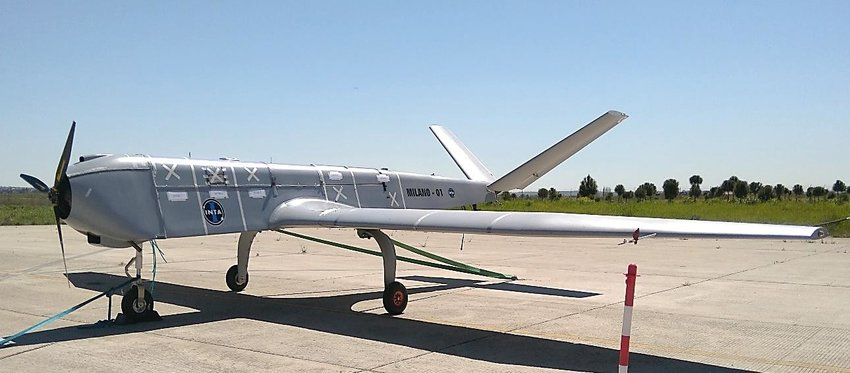
\includegraphics[width=120mm]{3/Fotos/Milano.png}
    \captionsetup{justification=centering,margin=1.25cm}
    \caption{UAV INTA Milano}
    \label{mialno}
\end{figure}


%----------%


\subsection{Estructura y red de sensores}

La estructura de la aeronave sobre la que se ha realizado el FEM y se ha fabricado después es el fuselaje posterior del UAV Milano. Esta estructura está compuesta por:

\begin{itemize}
    \item[\tiny$\bullet$] Revestimiento inferior con un larguero longitudinal en T dividido en dos y refuerzos sobre las pestañas. Fabricado con cinta UD fuera de autoclave.
    \item[\tiny$\bullet$] Revestimiento superior con dos largueros en L y refuerzos sobre las pestañas. Fabricado con cinta UD fuera de autoclave.
    \item[\tiny$\bullet$] Cuatro cuadernas con refuerzos sobre las mismas. Fabricadas con cinta UD fuera de autoclave.
    \item[\tiny$\bullet$] Dimensiones aproximadas de $2600 x 850 x 890$ mm.
\end{itemize}

En la Figura \ref{estructura_fuselaje} se puede ver el diseño explosionado de los componentes descritos.

\begin{figure}[ht!]
    \centering
    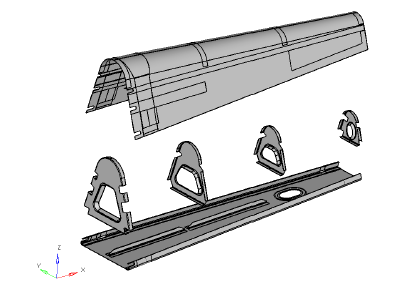
\includegraphics[width=130mm]{3/Fotos/estructura_fuselaje.png}
    \captionsetup{justification=centering,margin=1.25cm}
    \caption{Fuselaje posterior}
    \label{estructura_fuselaje}
\end{figure}

Sobre esta estructura se van a distribuir dos redes de sensores de fibra óptica, uno formado por sensores FBG y otro por OBR. Con ellos se recogerá el campo de deformaciones de la estructura que se procesará para obtener la clasificación de los daños. En las Figuras \ref{FBG_sensores} y \ref{OBR_sensores} se tiene una representación gráfica de la posición de estas redes en la estructura.

\begin{figure}[ht]
    \centering
    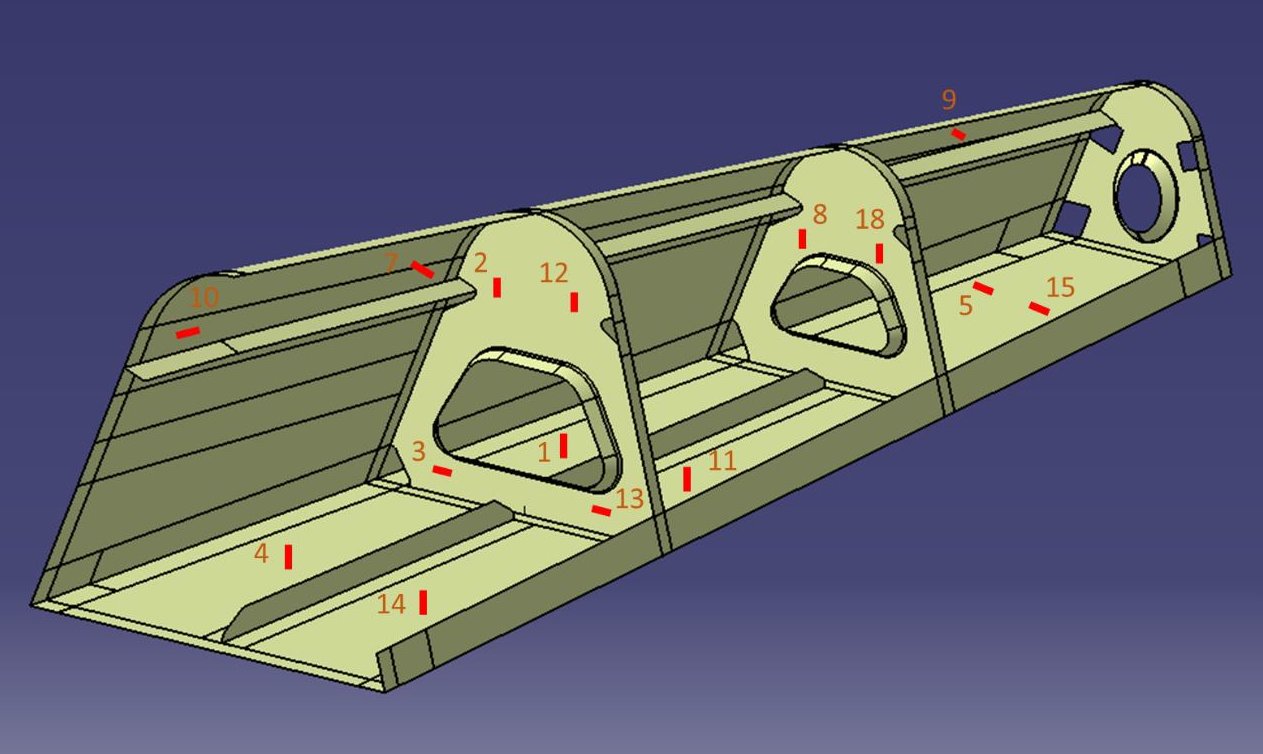
\includegraphics[width=125mm]{3/Fotos/FBG.png}
    \captionsetup{justification=centering,margin=1.25cm}
    \caption{Red de sensores FBG}
    \label{FBG_sensores}
\end{figure}

\begin{figure}[ht!]
    \centering
    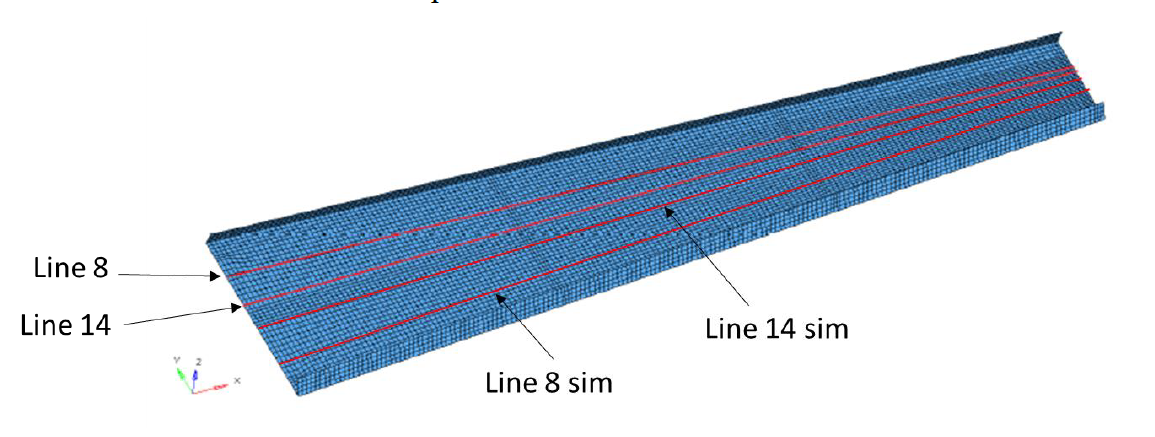
\includegraphics[width=130mm]{3/Fotos/OBR_1.png}
    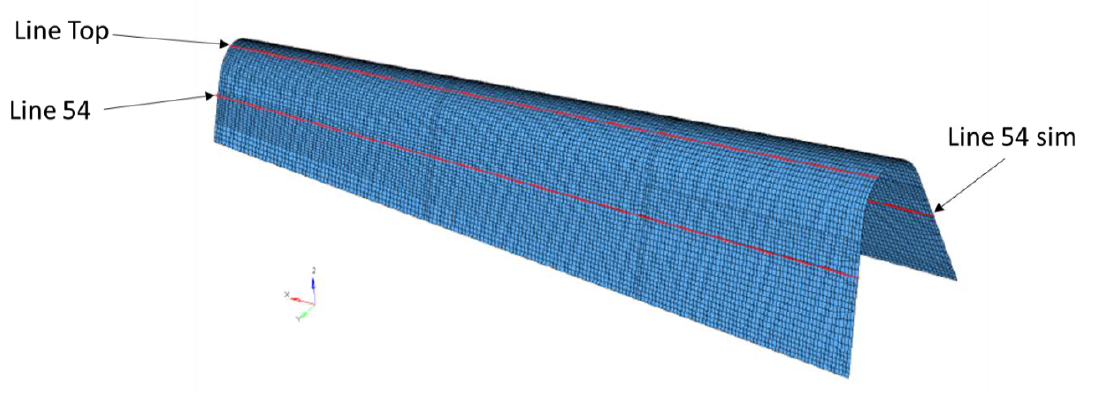
\includegraphics[width=130mm]{3/Fotos/OBR_2.png}
    \caption{Red de sensores OBR}
    \label{OBR_sensores}
\end{figure}

Es importante indicar que, puesto que los sensores de medida distribuida son unidireccionales, se han obtenido las deformaciones en la dirección longitudinal de la fibra (tracción/compresión).

%----------%

\subsection{Planteamiento de daños y descripción de ensayos} 

El objetivo de este proyecto es tener un sistema SHM para detectar daños en un fuselaje de material compuesto durante su operación, por lo tanto, se necesita definir la localización de estos daños y sus tamaños.

Estos daños corresponden con desencolados parciales o totales en las zonas que se definirán a continuación. En la Figura \ref{dam} se puede ver la localización de cada daño en la estructura y en la Tabla \ref{tdam} se pueden ver sus caracterísitcas.

\begin{figure}[ht]
    \centering
    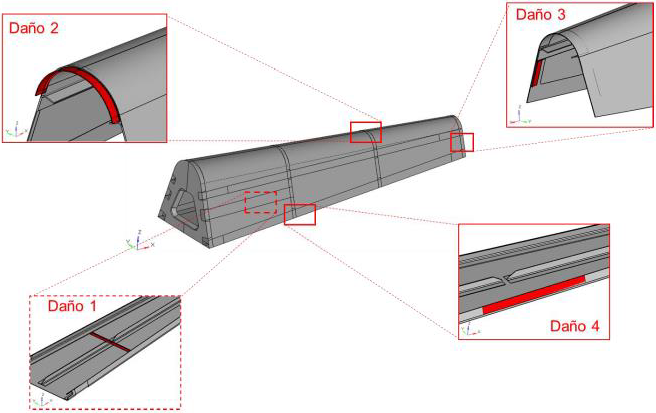
\includegraphics[width=125mm]{3/Fotos/dam.png}
    \caption{Esquema de los daños realizados a la estructura}
    \label{dam}
\end{figure}

\begin{table}[h!]
    \centering
    \begin{tabular}{ | m{12.5mm} | m{37.5mm}| m{30mm} |  m{25mm} |  m{25mm} |}  \hline
        \textbf{\footnotesize{DAÑO}}& \textbf{\footnotesize{TIPO DE DAÑO}} & \textbf{\footnotesize{ELEMENTOS AFECTADOS}} & \textbf{\footnotesize{LONGITUD MÁXIMA}} & \textbf{\footnotesize{INCREMENTO}}\\ 
        \hline
        D1 & Desencolado parcial del pie de la cuaderna & Cuaderna 2, revestimiento inferior & 450 mm & 30 mm \\ 
        \hline
        D2 & Desencolado parcial de la pestaña superior de la cuaderna & Cuaderna 3, revestimiento superior & 350 mm & 25 mm \\ 
        \hline
        D3 & Desencolado parcial de la pestaña lateral de la cuaderna & Cuaderna 4, revestimiento superior & 180 mm & 30 mm \\ 
        \hline
        D4 & Desencolado parcial entre el revestimiento inferior y el revestimiento superior & Revestimiento inferior, revestimiento superior & 900 mm & 30 mm \\ 
        \hline
    \end{tabular}
    \caption{Definición de daños en el fuselaje}
    \label{tdam}
\end{table}

Es importante resaltar que, aunque el ensayo estructural y las simulaciones se realizaron para los cuatro daños, se llegó a la conclusión de que el daño 3 era irrelevante tras ver los resultados obtenidos. Por lo tanto, dicho daño fue descartado.\\

Para facilitar el trabajo a los operarios que realizaron los ensayos del fuselaje, se sustituyó la unión adhesiva por uniones remachadas. Esto permitió controlar mejor la progresión de los daños y también que fueran reparados tal y como se ve en la Figura \ref{remaches}.

\begin{figure}[ht]
    \centering
    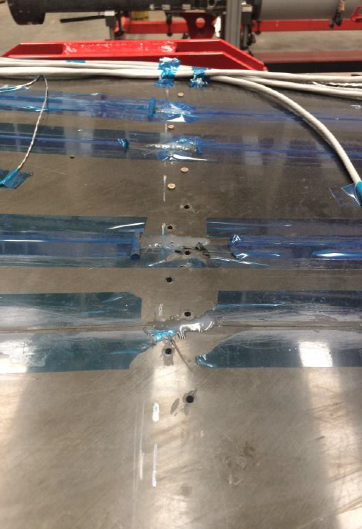
\includegraphics[width=55mm]{3/Fotos/remaches.png}
    \captionsetup{justification=centering,margin=1.25cm}
    \caption{Realización del daño por extracción de remaches}
    \label{remaches}
\end{figure}

Los ensayos sobre la estructura real se simularon también siguiendo la misma configuración en el FEM. Las condiciones de contorno a las que está sometido el fuselaje son las siguientes:

\begin{itemize}
    \item[\tiny$\bullet$] Empotramiento en la sección de unión con el fuselaje anterior
    \item[\tiny$\bullet$] Carga vertical en la sección de unión con la cola
\end{itemize}

El ensayo comienza con la estructura descargada y se aplica la carga de forma escalonada. La carga va aumentando 400 N en 10 escalones hasta llegar a un máximo de 4 kN.

La configuración del banco de ensayos se puede ver en la Figura \ref{ensayo}

\begin{figure}[ht]
    \centering
    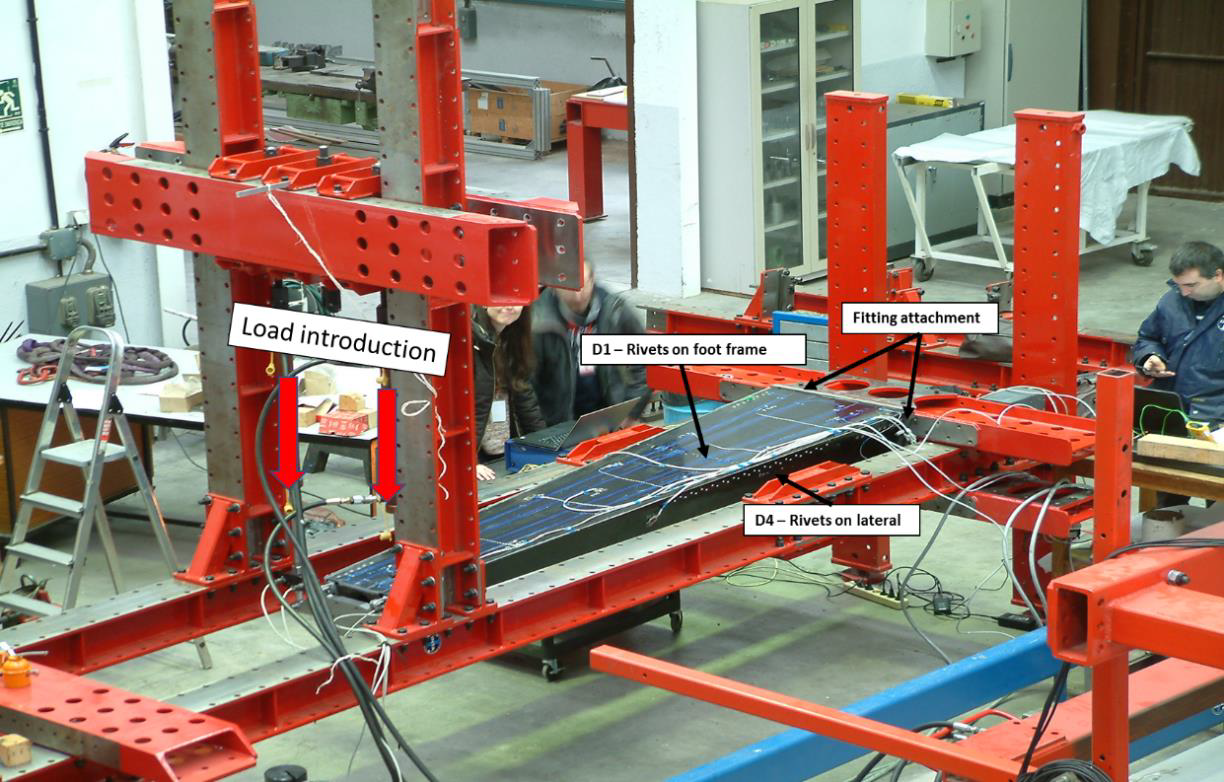
\includegraphics[width=145mm]{3/Fotos/ensayo.png}
    \captionsetup{justification=centering,margin=1.25cm}
    \caption{Vista general de la configuración de los ensayos}
    \label{ensayo}
\end{figure}


%----------%


\subsection{Modelo de elementos finitos}

Se va a hacer un breve resumen de las características del FEM utilizado. Este modelo consta de 62802 grados de libertad, el tamaño medio de sus elementos es de 15 mm, y está formado por:
\begin{itemize}
    \item[\tiny$\bullet$] 26181 nodos
    \item[\tiny$\bullet$] 34080 elementos quad4 (Ratio máximo de 4.768)
    \item[\tiny$\bullet$] 25 elementos tria3 (Ratio máximo de 6.219)
\end{itemize}

Los elementos tria3 del modelo se encuentran principalmente en las cuatro cuadernas debido a que su geometría es más complicada de mallar que la del resto del fuselaje.\\

En la Figura \ref{femest} se pueden ver los distintos elementos del modelo y en cuales de ellos se introducen las condiciones de contorno.

\begin{figure}[h!]
    \centering
    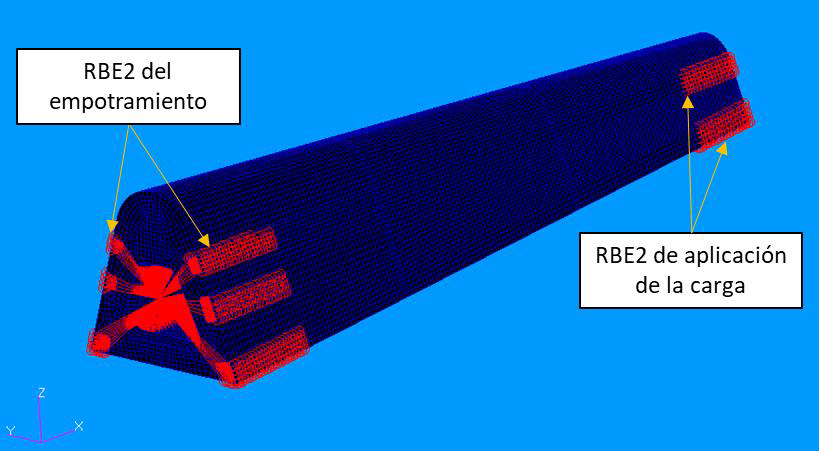
\includegraphics[width=120mm]{3/Fotos/femest.png}
    \captionsetup{justification=centering,margin=1.25cm}
    \caption{Modelo de elementos finitos del fuselaje posterior del UAV Milano}
    \label{femest}
\end{figure}


%----------%

\clearpage

\section{Pre-procesado de señales}

Una vez que se han realizado los ensayos y simulaciones, es necesario pre-procesar los datos recogidos por las redes de sensores para ajustarlos en contenido y forma para que las redes neuronales puedan realizar una clasificación correcta.

Los datos que se obtienen de los ensayos reales se van a tratar de forma diferente a los obtenidos a través del FEM, por ello, este apartado está separado en dos grupos, \textit{Ensayo real} y \textit{FEM}.

\subsection{Ensayo real}
    
La red de sensores FBG registra las deformaciones de forma ininterrumpida durante el ensayo completo, dando así una curva de deformación frente al tiempo para cada uno de los sensores distribuidos en la estructura, como se puede ver a continuación en la Figura \ref{def_t}.\\
    
\begin{figure}[h!]
    \centering
    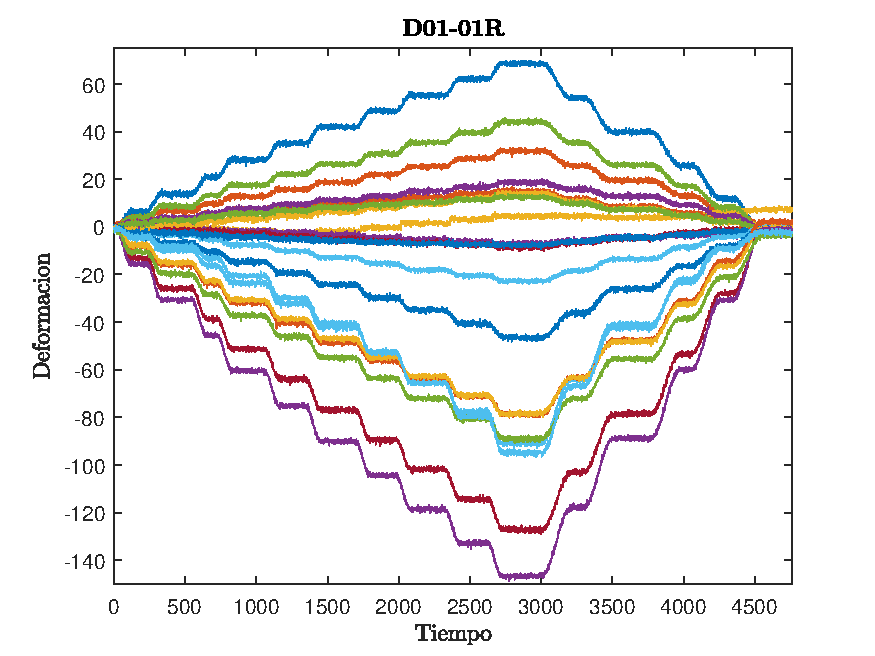
\includegraphics[width=125mm, angle=0]{3/Fotos/Sensores_FBG.pdf}
    \captionsetup{justification=centering,margin=1.25cm}
    \caption{Medida de todos los sensores durante el ensayo del Daño 1 con un remache extraído}
    \label{def_t}
\end{figure}
    
Cuando los actuadores llegan a un nivel de carga paran durante un tiempo antes de aumentar o disminuir la carga aplicada con el fin de estabilizar la carga. Por lo tanto, para separar las medidas en diferentes niveles de carga hay que detectar cuando el actuador comienza a moverse. La detección de el comienzo de aplicación de carga está representada en las Figuras \ref{def_s} y \ref{def_p}.
    
\begin{figure}[h!]
    \centering
    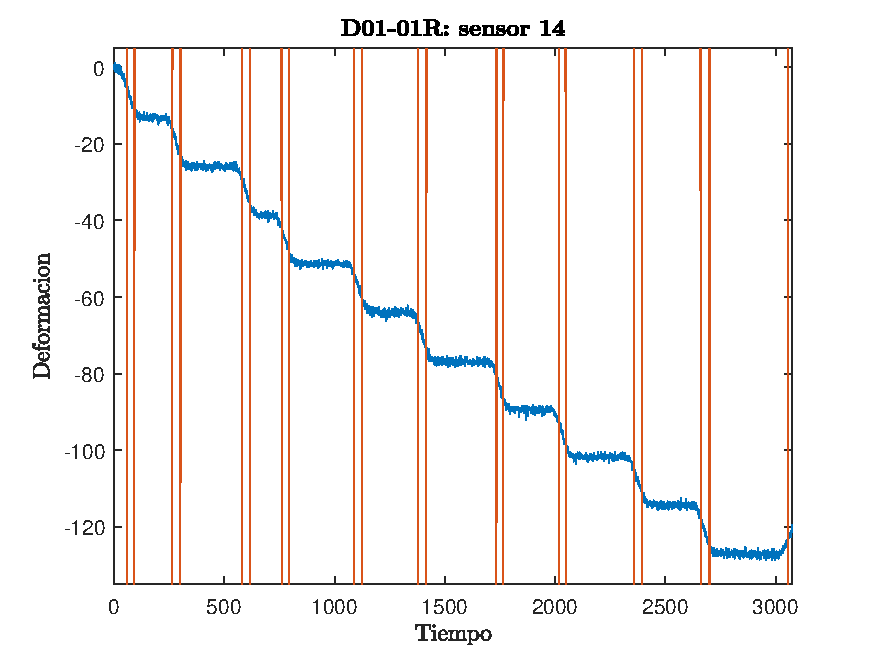
\includegraphics[width=125mm, angle=0]{3/Fotos/Saltos_FBG.pdf}
    \captionsetup{justification=centering,margin=1.25cm}
    \caption{Detección de los escalones producidos por las carga vertical}
    \label{def_s}
\end{figure}
    
\begin{figure}[h!]
    \centering
    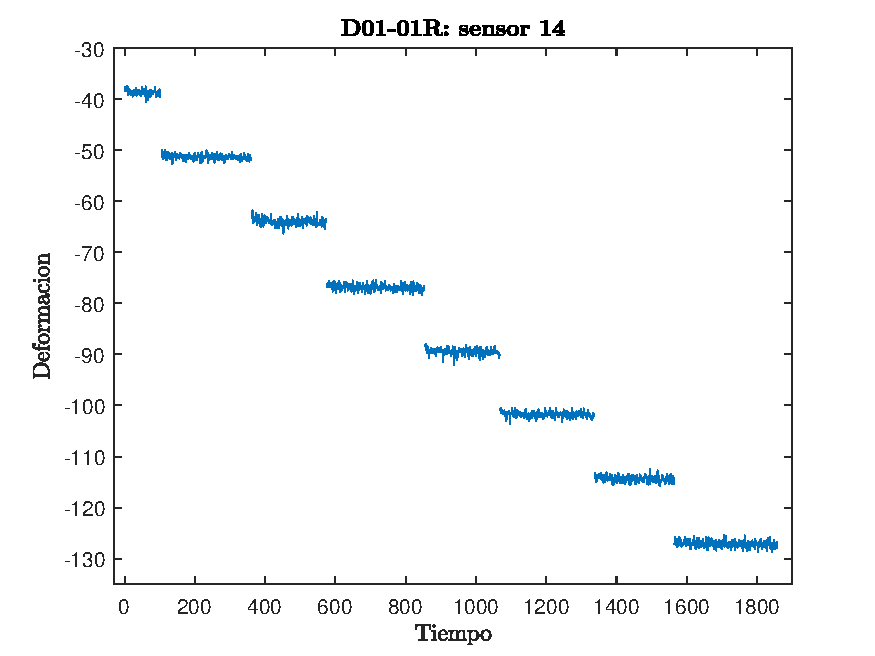
\includegraphics[width=125mm, angle=0]{3/Fotos/Procesado_FBG.pdf}
    \captionsetup{justification=centering,margin=1.25cm}
    \caption{Medidas de los sensores FBG en el ensayo preprocesadas}
    \label{def_p}
\end{figure}    
    
Finalmente se eliminan las medidas obtenidas durante la transición entre escalones usando como referencia las líneas naranjas de la Figura \ref{def_s} y se fija la carga mínima que se va a usar durante el estudio en un 30\% de la carga máxima.\\
 %Tras este proceso se obtienen múltiples ensayos individuales para cada carga y tipo de daño tal y como se ve en la Figura \ref{def_p}.
    
Una vez que se han aislado los escalones se dibuja un histograma para ver la variabilidad de los datos obtenidos. Como se ve en la Figura \ref{def_h}, los valores de las medidas se asemejan a una distribución normal con mida -127.75 deformaciones. Esto quiere decir que el ruido introducido por los sensores FBG hace que cada medida que se realiza en un tiempo diferente pueda ser considerada como un ensayo independiente. De un único ciclo de carga se obtienen una gran cantidad de datos para entrenar a la red.\\

\begin{figure}[h!]
    \centering
    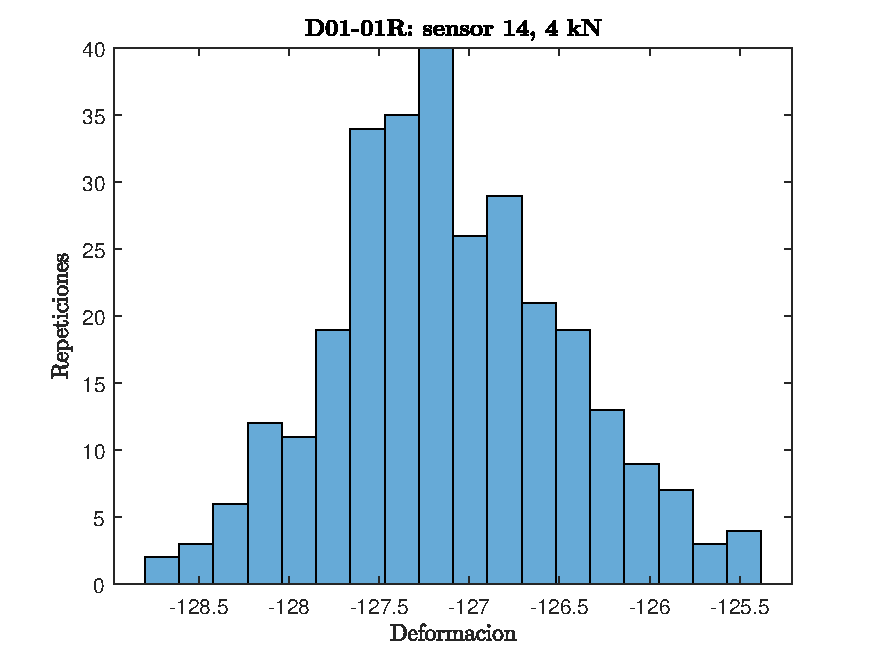
\includegraphics[width=125mm, angle=0]{3/Fotos/Histograma_FBG.pdf}
    \captionsetup{justification=centering,margin=1.25cm}
    \caption{Histograma del escalón 4 kN, 100\% de carga}
    \label{def_h}
\end{figure}    

Tras pre-procesar las señales se puede visualizar el campo de deformaciones medido por los sensores FBG para cada estado de daño y el estado sin daño o de referencia en la Figura \ref{FBGR_dam}. Al estar cada daño localizado en una zona diferente de la estructura, los cambios en el campo de deformaciones son locales y en la Figura \ref{FBGR_dif} se aprecia que sensores están más cerca de la zona dañada ya que sufren una mayor variación respecto a las medidas obtenidas de la estructura sin daño.

\begin{figure}[h!]
    \centering
    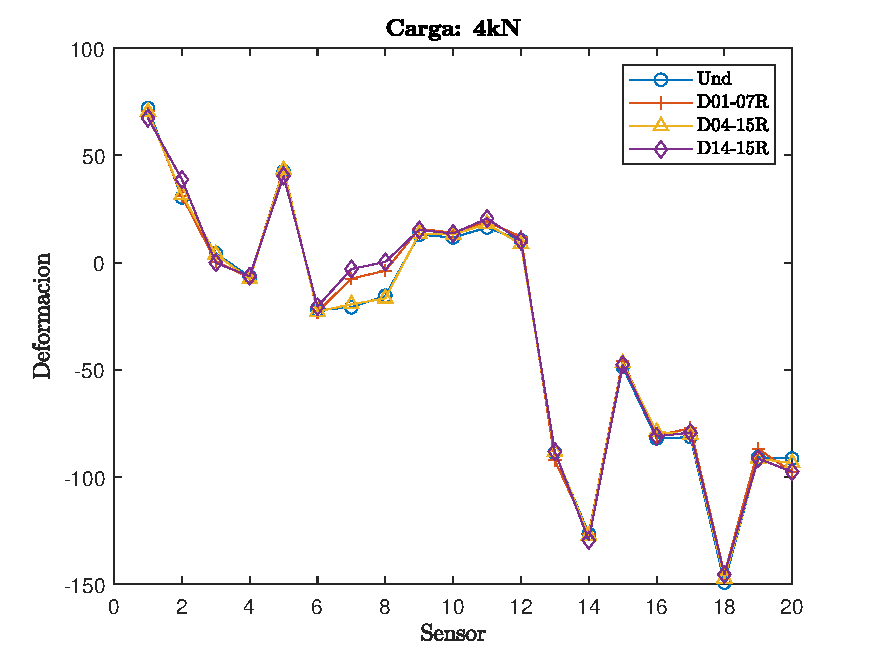
\includegraphics[width=125mm, angle=0]{3/Fotos/FBG_damages.pdf}
    \captionsetup{justification=centering,margin=1.25cm}
    \caption{Campo de deformaciones medido por los sensores FBG para todos los daños}
    \label{FBGR_dam}
\end{figure}
        
\begin{figure}[h!]
    \centering
    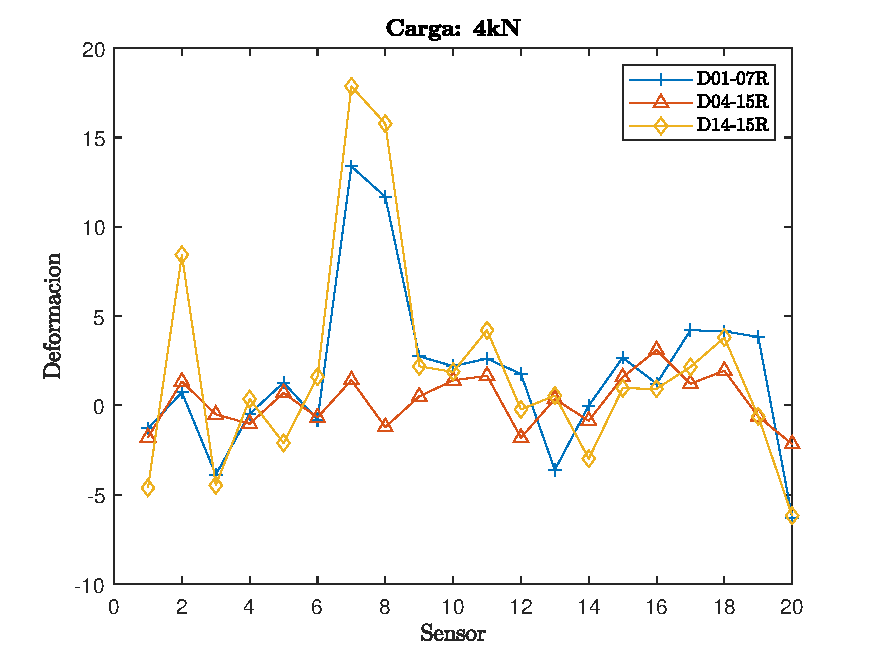
\includegraphics[width=125mm, angle=0]{3/Fotos/FBG_dif.pdf}
    \captionsetup{justification=centering,margin=1.25cm}
    \caption{Diferencia de los campos de deformaciones referenciado con el estado sin daño (FBG)}
    \label{FBGR_dif}
\end{figure}


%----------------------%

    

\vspace*{10pt}
    
Por otro lado, los sensores OBR realizan una captura instantánea del campo de deformaciones. Esto quiere decir que se tiene una única muestra para cada tipo de daño y nivel de carga (ejemplo en la Figura \ref{fig:D01-R3}), lo cual es insuficiente para conseguir unos buenos resultados con la red.\\

\begin{figure}[h!]
    \centering
    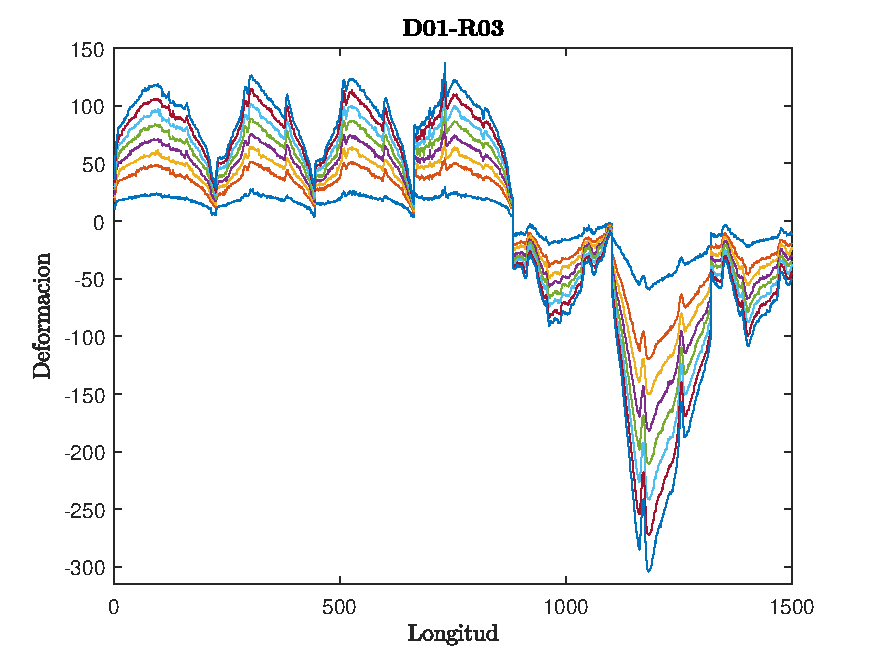
\includegraphics[width=125mm, angle=0]{3/Fotos/D01-R3.pdf}
    \captionsetup{justification=centering,margin=1.25cm}
    \caption{Campo de deformaciones provocado por el daño 1 con 3 remaches extraídos para todos los casos de carga}
    \label{fig:D01-R3}
\end{figure}
    
Siguiendo el mismo razonamiento usado con los sensores FBGs, si se añade una distribución de ruido gausiano a un valor del campo de deformaciones, se pueden generar ensayos independientes con los que entrenar a la red. Sin embargo, el campo de deformaciones de la Figura \ref{fig:D01-R3} ya contiene ruido asociado a la medida. 

Para conseguir un campo de deformaciones que usar como referencia, al que añadir posteriormente ruido, se va a utilizar el filtro \textit{Savitzky-Golay}. Este filtro digital es comúnmente usado para suavizar series de datos equiespaciados \cite{Savitzky-Golay}.

\begin{figure}[h!]
    \centering
    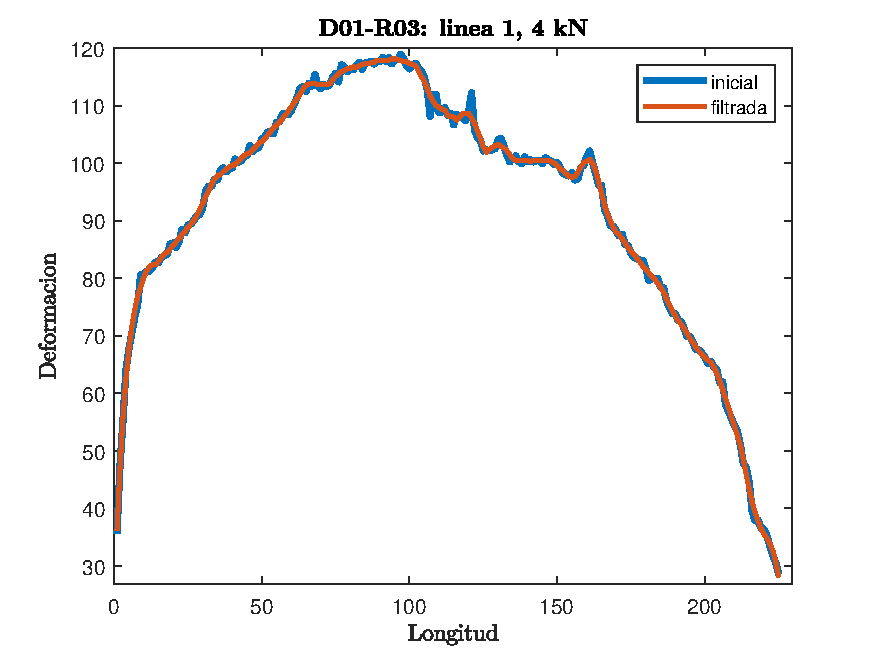
\includegraphics[width=125mm, angle=0]{3/Fotos/filtro.pdf}
    \captionsetup{justification=centering,margin=1.25cm}
    \caption{Aplicación del filtro Savitzky-Golay a una linea de sensor OBR}
    \label{fig:filtro}
\end{figure}

La diferencia entre la medida sin filtrar y filtrada se aprecia claramente en la Figura \ref{fig:filtro}.\\

Ahora que se tiene una medida de referencia, ya se puede añadir la distribución de ruido de amplitud 1.5 deformaciones (Figura \ref{OBRR_ruido}) y generar más muestras.
    
\begin{figure}[h!]
    \centering
    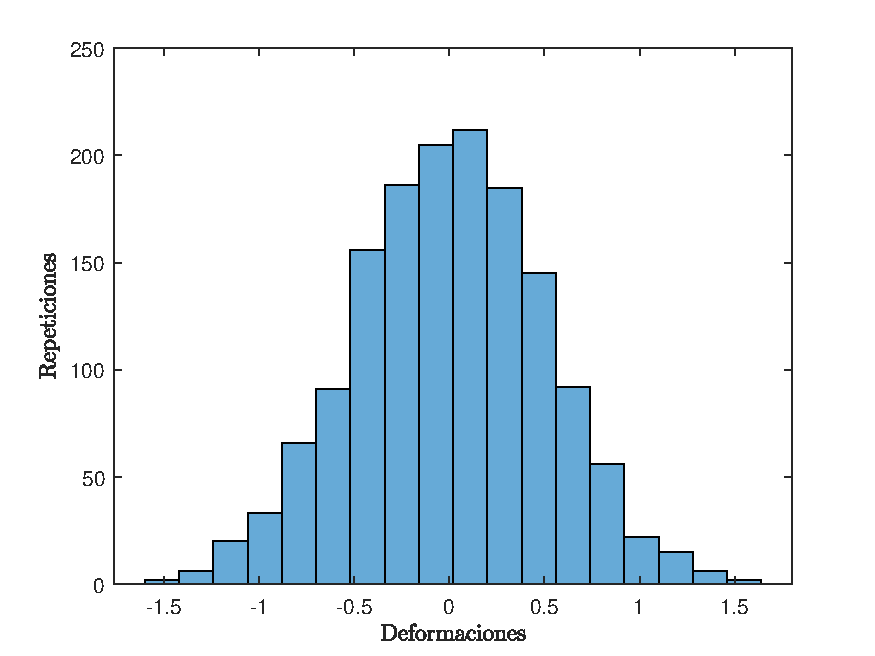
\includegraphics[width=125mm, angle=0]{3/Fotos/histo_ruido_OBR.pdf}
    \captionsetup{justification=centering,margin=1.25cm}
    \caption{Distribución de ruido gausiano con amplitud 1.5 deformaciones}
    \label{OBRR_ruido}
\end{figure}
    
En la Figura \ref{fig:OBRR_det} se puede ver un detalle del caso D01-R03 en el que se ha ampliado las deformaciones medidas por una línea de sensor. Aquí se aprecia más claramente que cada una de estas muestras se pueda considerar como un ensayo independiente.
    
\begin{figure}[h!]
    \centering
    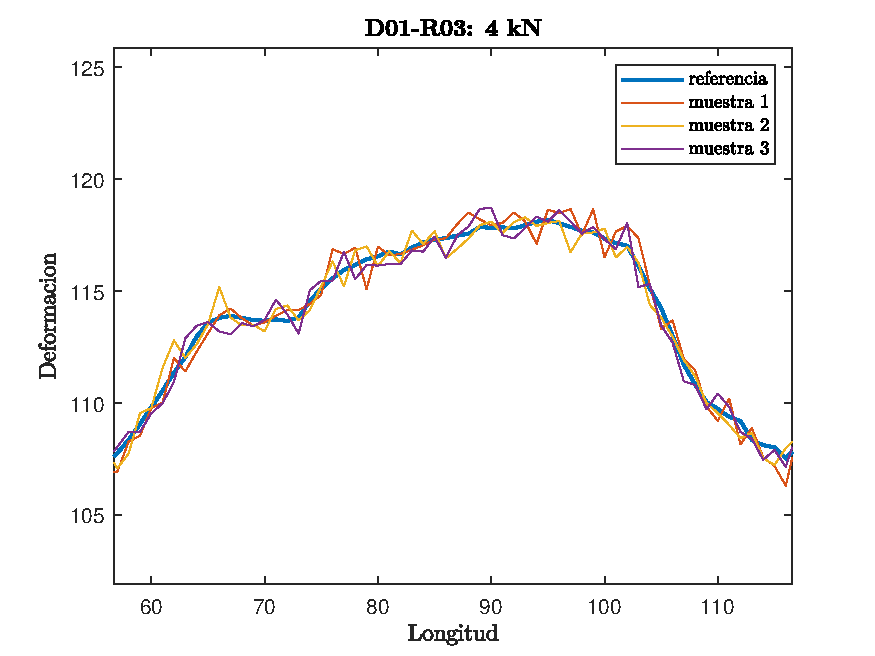
\includegraphics[width=125mm, angle=0]{3/Fotos/detalle_OBR_ruido.pdf}
    \captionsetup{justification=centering,margin=1.25cm}
    \caption{Detalle de las variaciones provocadas por el ruido gausiano}
    \label{fig:OBRR_det}
\end{figure}
   
Igual que se ha hecho con los FBGs, en las Figuras \ref{OBRR_dam} y \ref{OBRR_dif} se pueden ver los campos de deformaciones provocados por los distintos daños con la carga máxima y su diferencia respecto al estado sin daño.

\begin{figure}[h!]
    \centering
    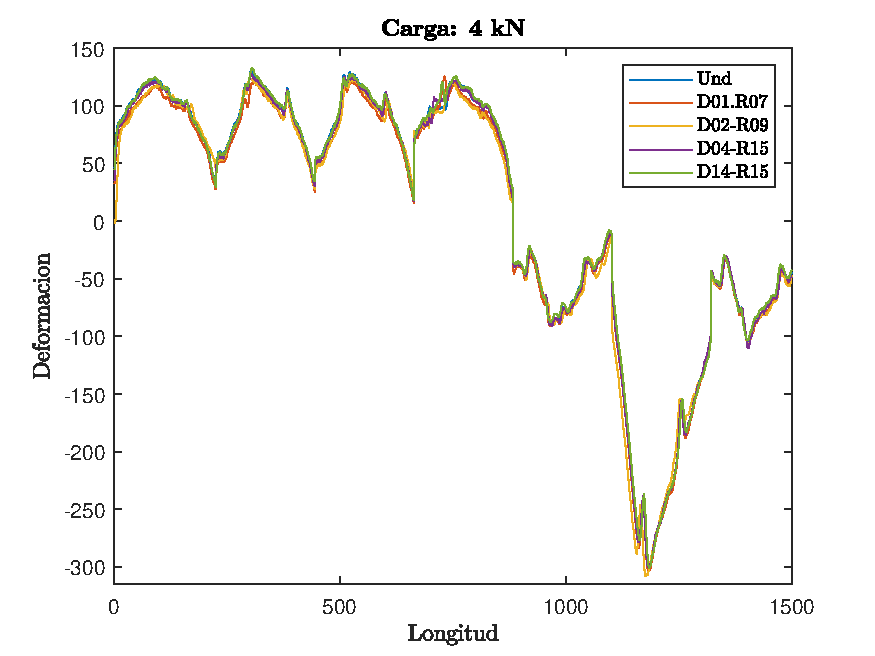
\includegraphics[width=125mm, angle=0]{3/Fotos/OBR_damages.pdf}
    \captionsetup{justification=centering,margin=1.25cm}
    \caption{Campo de deformaciones medido por el sensor OBR para todos los daños}
    \label{OBRR_dam}
\end{figure}
    
\begin{figure}[h!]
    \centering
    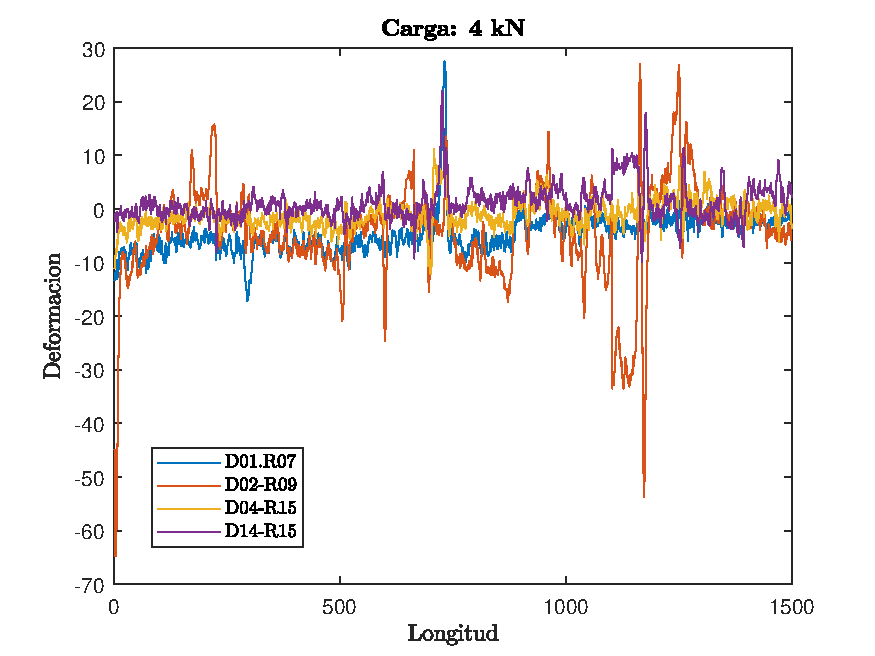
\includegraphics[width=125mm, angle=0]{3/Fotos/OBR_dif.pdf}
    \captionsetup{justification=centering,margin=1.25cm}
    \caption{Diferencia de los campos de deformaciones referenciado con el estado sin daño (OBR)}
    \label{OBRR_dif}
\end{figure}


\url{https://towardsdatascience.com/hands-on-graph-neural-networks-with-pytorch-pytorch-geometric-359487e221a8}

\clearpage


%  -----------------------------------------  %


\section{Aplicación de DL al a la detección de daños mediante sensores de deformaciones}

\subsection{Visualización del campo de deformaciones}

Una vez que se han procesado las deformaciones se tiene un \textit{Dataset} para los sensores FBG en el que cada muestra es de dimensión 20 (20 sensores) mientras que en el dataset de los sensores OBR las muestras son de dimensión 1499 (equivalente a tener 1499 sensores).

Un ser humano no puede visualizar un espacio con tantas dimensiones. Esto hace complicado tener una idea de la distribución espacial de las muestras y mucho menos imaginar las fronteras que genera la NN entre las distintas clases de datos (como se ha explicado en \hyperref[sec:funcionamiento_DL]{\textit{Representación gráfica del funcionamiento una NN}}).\\

Para reducir la dimensionalidad de los datasets y tener una representación gráfica bidimensional de ellos se va a utilizar un algoritmo de Machine Learning muy popular para la visualización de datos multidimansionales: \textbf{t-SNE (t-distributed Stochastic Neighbor Embedding)}. A continuación se va a hacer una breve introducción al funcionamiento de este algoritmo extraído de \cite{t_sne}.\\

\textit{Stochastic Neighbor Embedding (SNE)} comienza convirtiendo las distancias euclideas entre puntos del dataset de alta dimensionalidad en probabilidades condicionales que representan su similitud. La similitud del punto $x_j$ con el punto $x_i$ es la probabilidad condicional $p_{j|i}$ y su proximidad se calcula usando una distribución de densidad de probabilidad gaussiana centrada en $x_i$. Para los puntos cercanos, el $p_{j|i}$ es relativamente alto, mientras que para los puntos lejanos, el $p_{j|i}$ será casi infinitesimal. Matemáticamente, el la probabilidad condicional $p_{j|i}$ viene dada por la Ecuación \ref{eq:prob_alta}.

\begin{equation}
	p_{j|i} = \frac{exp(-||x_i-x_j||^2/2\sigma ^2_i)}{\sum_{k\neq i}( exp(-||x_i-x_k||^2/2\sigma ^2_i)}
	\label{eq:prob_alta}
\end{equation}
\vspace{4pt}

En el espacio de baja dimensión los puntos $y_i$ y $y_j$ son la transformación de $x_i$ y $x_j$ del espacio con alta dimensionalidad. Es posible calcular una probabilidad condicional similar, $q_{j|i}$ a la anterior. Para ello, fijamos la varianza del gaussiano que se emplea en el cálculo de las probabilidades condicionales $q_{j|i}$ en $\frac{1}{\sqrt{2}}$. Por lo tanto, modelamos la similitud del punto $y_j$ con $y_i$ con la Ecuación \ref{eq:prob_baja}

\begin{equation}
	q_{j|i} = \frac{exp(-||y_i-y_j||^2)}{\sum_{k\neq i}(exp(-||y_i-y_k||^2)}
	\label{eq:prob_baja}
\end{equation}
\vspace{4pt}

Si los puntos $y_i$ y $y_j$ del mapa de baja dimensionalidad modelan bien la similaridad entre los puntos $x_i$ y $y_j$ del espacio con alta dimensionalidad, las probabilidades $p_{j|i}$ y $q_{j|i}$ serán iguales. Por lo tanto, el objetivo de SNE es minimizar las discordancias entre $p_{j|i}$ y $q_{j|i}$.\\

Igual que para las NN, es necesario tener una función de costes que represente el error que está cometiendo el algoritmo y así optimizarla por medio del descenso del gradiente. La función de costes elegida es la divergencia Kullback-Leibler individual entre las distribuciones de probabilidad conjunta, P y Q (Equación \ref{eq:costes}).

\begin{equation}
	C = KL(P||Q) = \sum_{i}\sum_{j}p_{ji}\log\frac{p_{j|i}}{q_{j|i}}
	\label{eq:costes}
\end{equation}
\vspace{4pt}

Para ambos sensores se va a visualizar la similitud entre los distintos tipos de daño, su tamaño y la la carga aplicada.

\begin{itemize}
    \item[$\bullet$] \textbf{Sensores FBG}

    \begin{figure}[H]
        \centering
        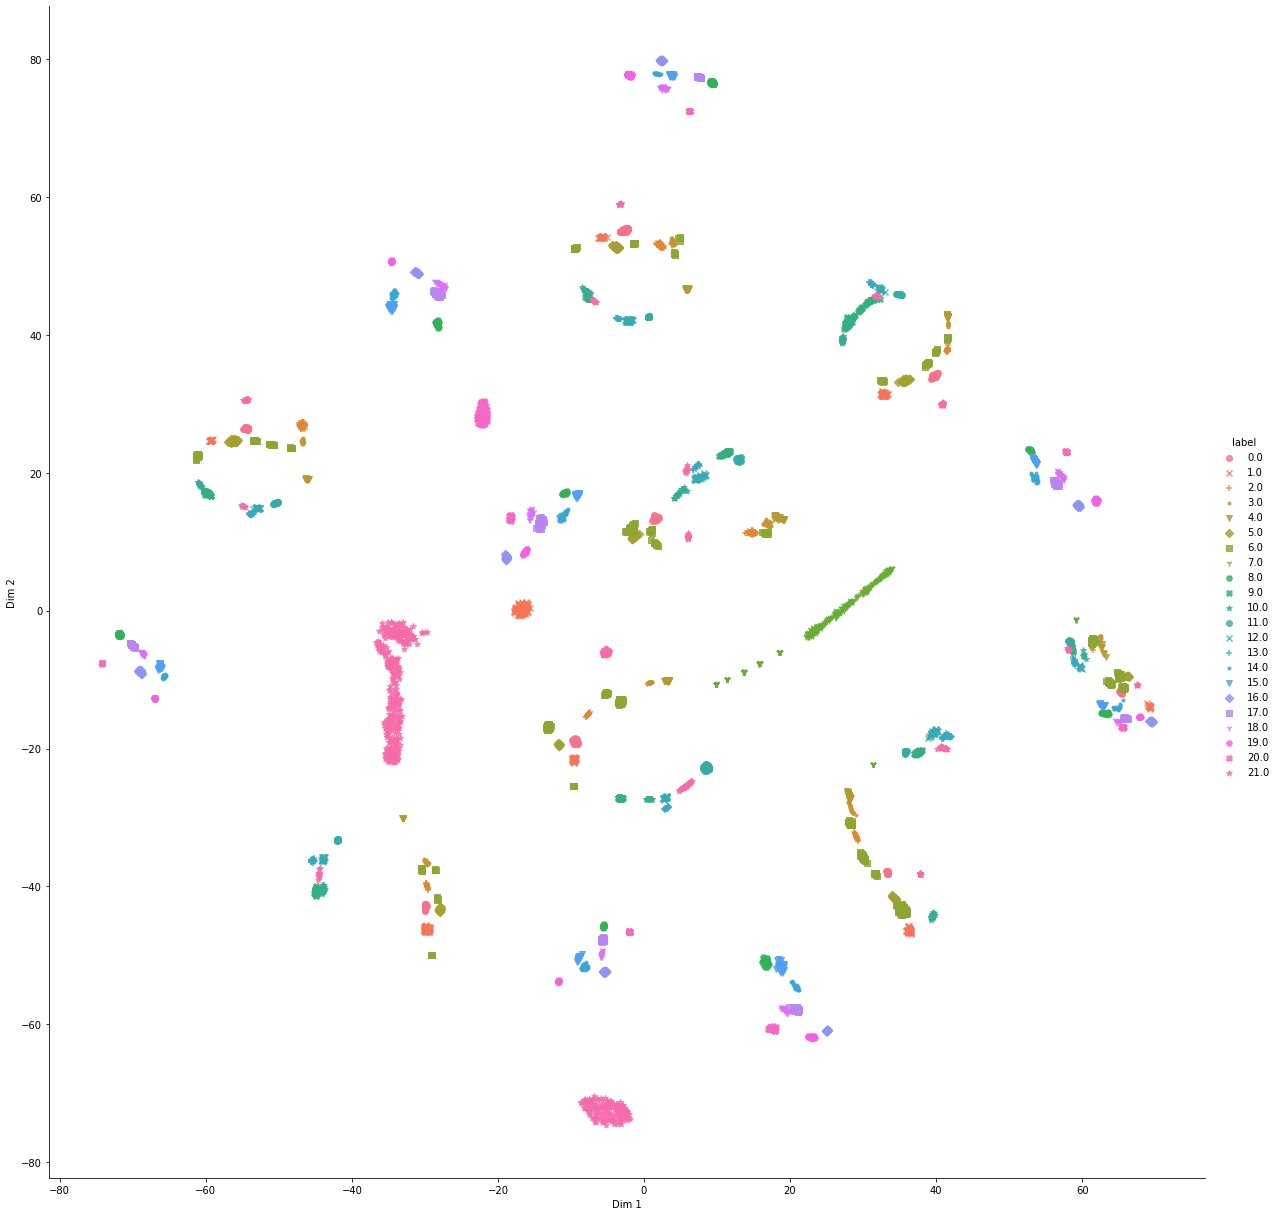
\includegraphics[width=125mm]{3/Fotos/Ty_Si_INESASSE_t-sne.png}
        \captionsetup{justification=centering,margin=1.25cm}
        \caption{Visualización de los distintos tamaños de daño}
        \label{fig:tsne_FBG_Ty_Si}
    \end{figure}  
    
    \begin{figure}[H]
        \centering
        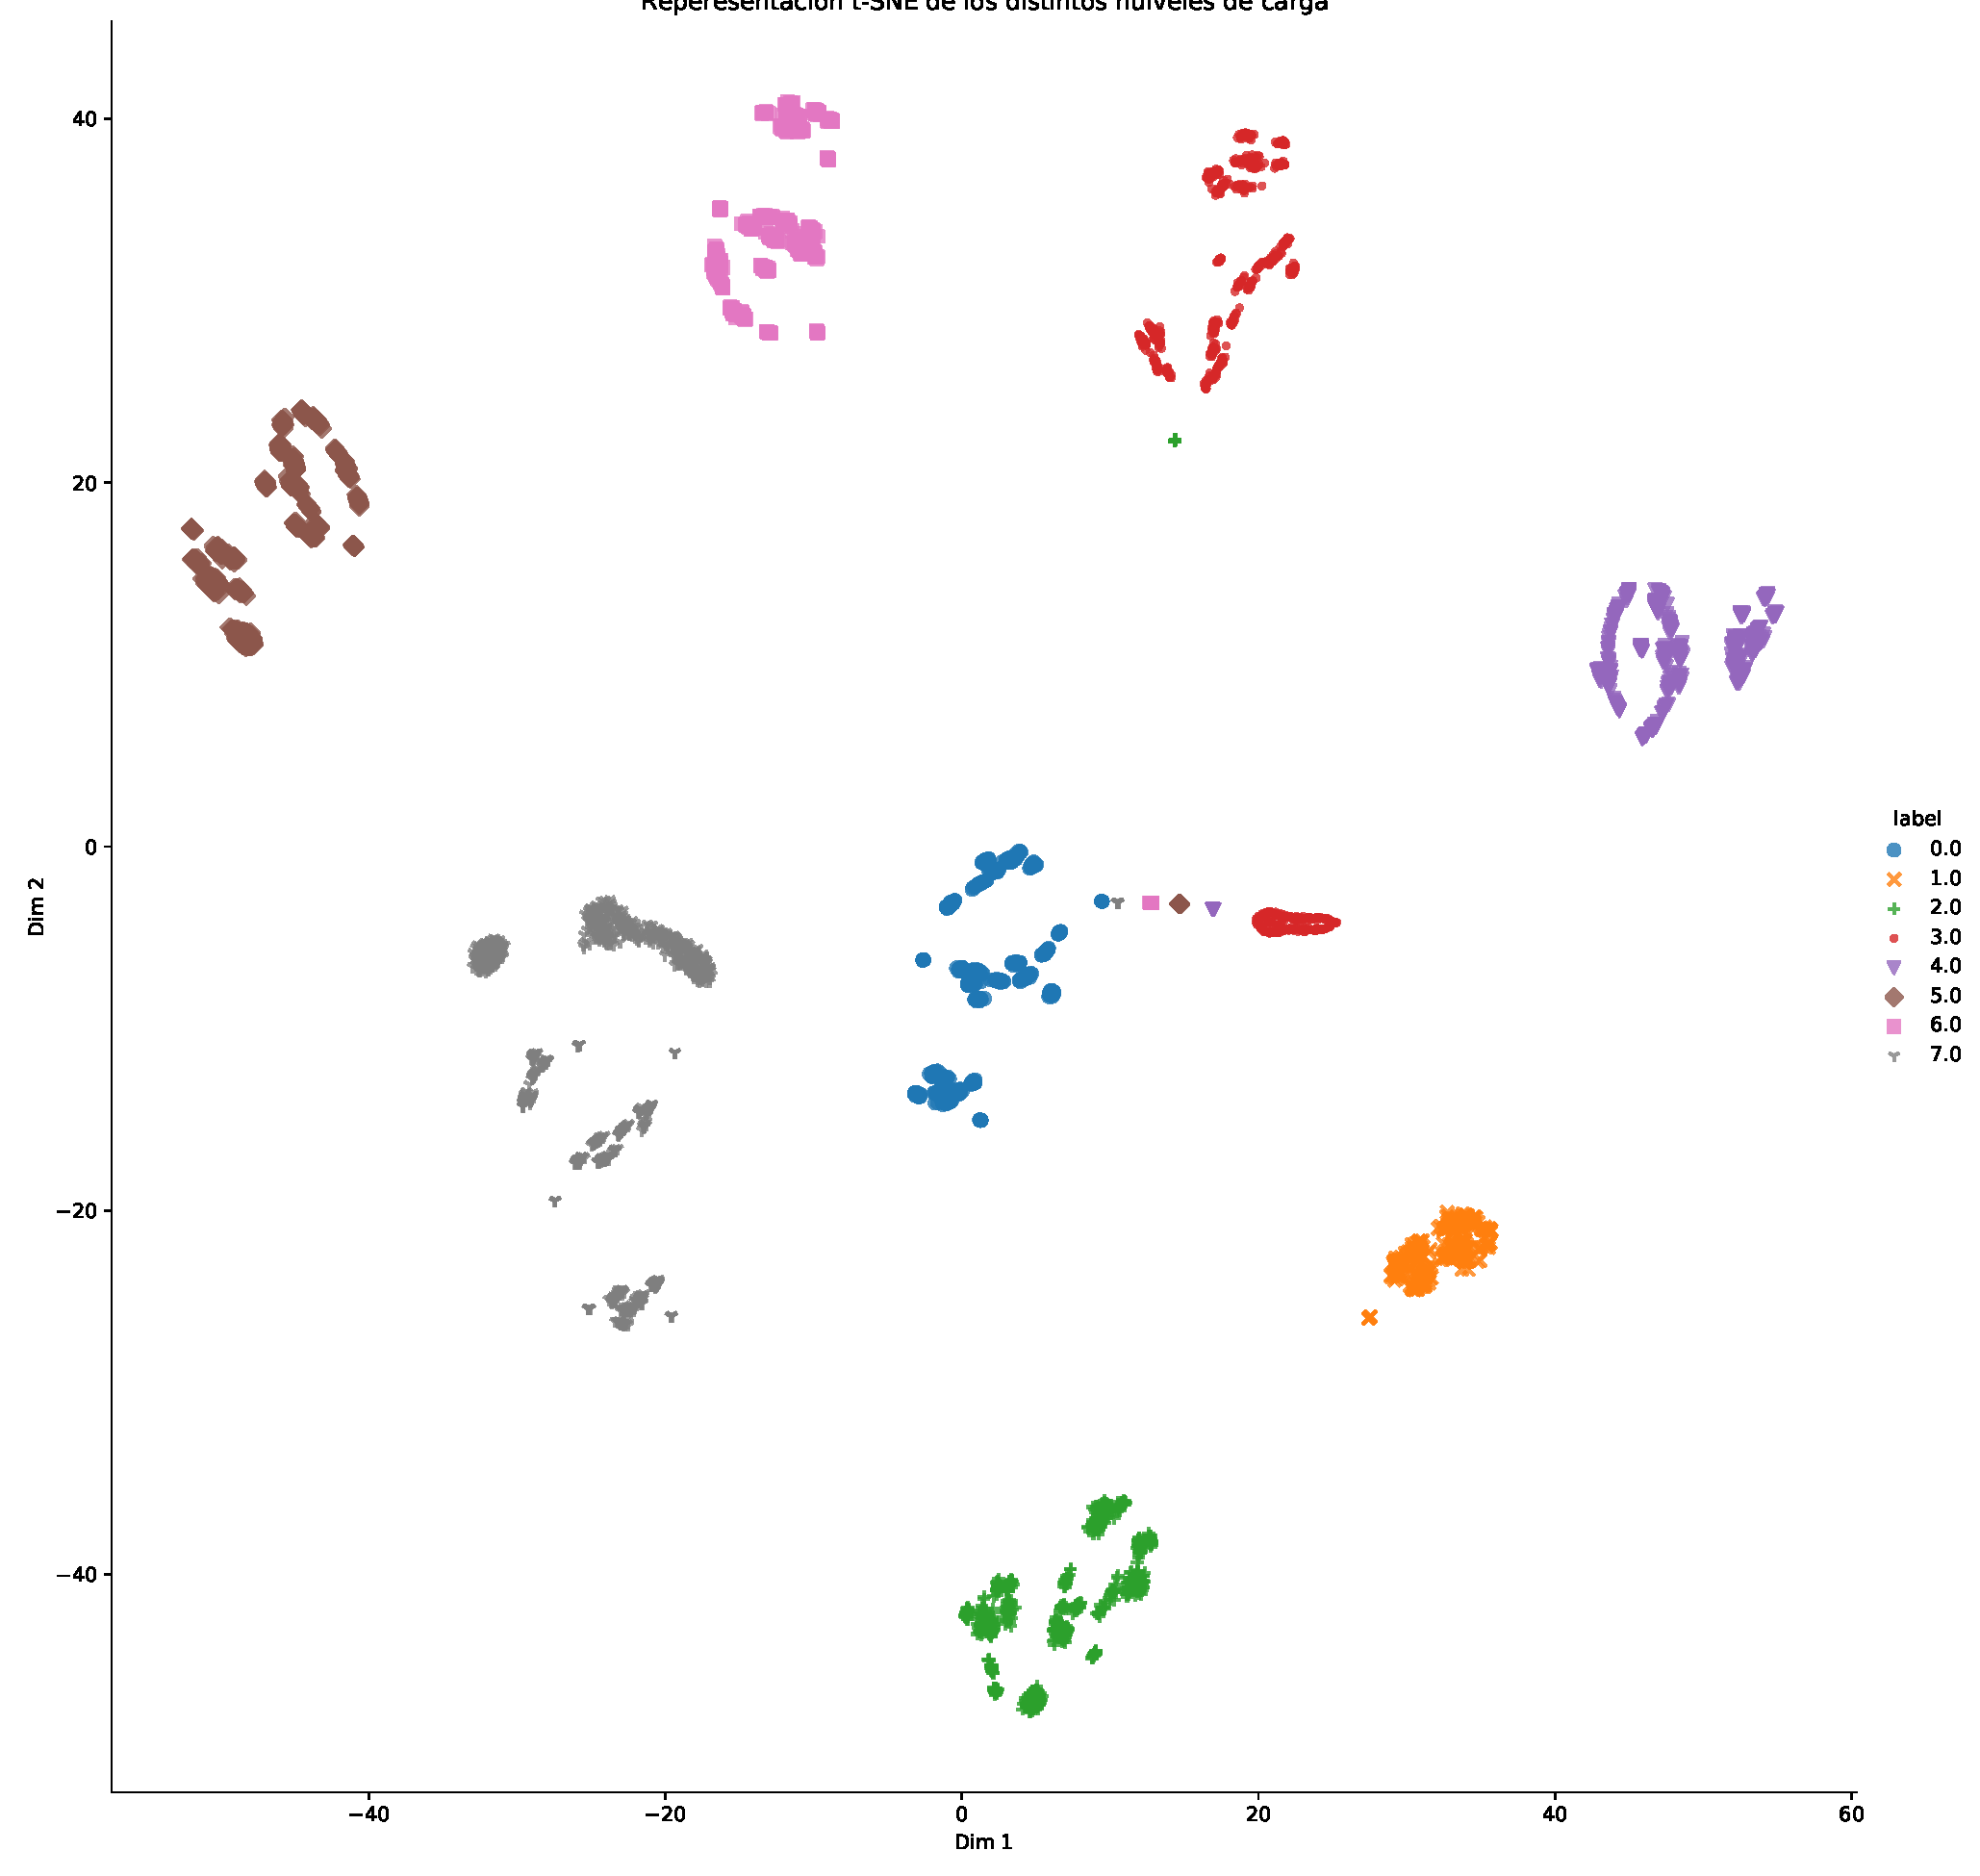
\includegraphics[width=125mm]{3/Fotos/tsne_Load_INESASSE.pdf}
        \captionsetup{justification=centering,margin=1.25cm}
        \caption{Visualización de los distintos niveles de carga}
        \label{fig:tsne_FBG_Load}
    \end{figure}  
    
	\item[$\bullet$] \textbf{Sensores OBR}    
    
    \begin{figure}[H]
        \centering
        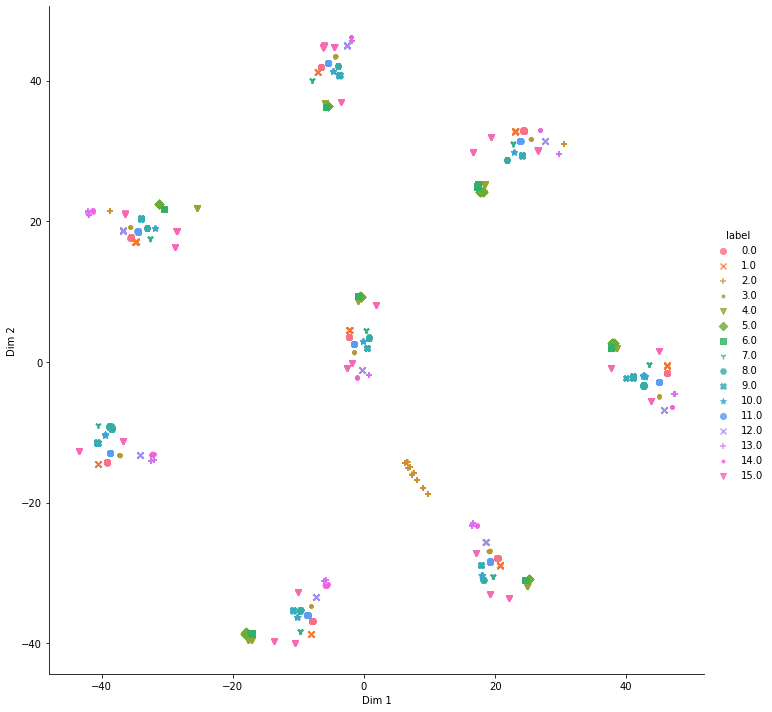
\includegraphics[width=125mm]{3/Fotos/tsne_Ty_Si_OBR_INESASSE.png}
        \captionsetup{justification=centering,margin=1.25cm}
        \caption{Visualización de los distintos tamaños de daño}
        \label{fig:tsne_OBR_Ty_Si}
    \end{figure}  
    
    \begin{figure}[H]
        \centering
        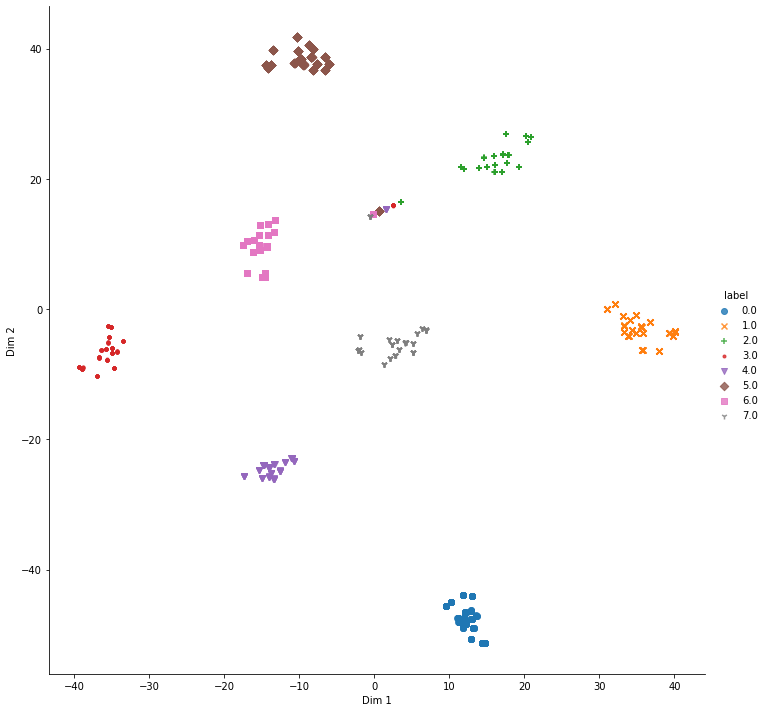
\includegraphics[width=125mm]{3/Fotos/tsne_Load_OBR_INESASSE.png}
        \captionsetup{justification=centering,margin=1.25cm}
        \caption{Visualización de los distintos niveles de carga}
        \label{fig:tsne_OBR_Load}
    \end{figure}      
    
    
\end{itemize}

Aquí se puede ver claramente en las Figuras \ref{fig:tsne_FBG_Load} y \ref{fig:tsne_FBG_Load} que las muestras que están sometidas a un mismo nivel de carga están próximas en el espacio y separadas de los otros \textit{clusters} que forman el resto de cargas. En las Figuras \ref{fig:tsne_FBG_Ty_Si} y \ref{fig:tsne_FBG_Ty_Si} también se ven pequeños clusters de cada tipo de daño repartidos en grupos más grandes correspondientes a los distintos niveles de carga. Por lo tanto, las muestras se separan en clusters de niveles de carga (claramente diferenciados) y dentro de cada carga, se agrupan por tipo y tamaño de daño.


\clearpage


% -- -- %


\subsection{Arquitectura de la Red Neuronal}

En este apartado se tiene que explicar la arquitectura escogida. Tengo que encontrar una forma buena de pintarlo.


% -- -- %


\subsection{Resultados de la clasificación}

Una buena forma de representar el funcionamiento de una NN en la tarea de clasificación es mediante el uso de Matrices de Confusión (CM).\\

En estas matrices, cada columna pertenece a una única clase. Al introducir un campo de deformaciones etiquetado como una clase en concreto (D01-R03), la red, después de realizar todas las operaciones definidas por su arquitectura, sacará una clase como output. Entonces, si se ha realizado una clasificación exitosa, la CM sumará en la columna D01-R03 y fila D01-R03 una unidad. Sin embargo, si clasifica erróneamente, sumará uno en una fila diferente. 

Por lo tanto, cuanto mayor sea el valor de las celdas de la diagonal principal de la CM, mejor realizará la red la tarea de clasificación.

\begin{itemize}
    \item[$\bullet$] \textbf{Sensores FBG}

    \begin{figure}[H]
        \centering
        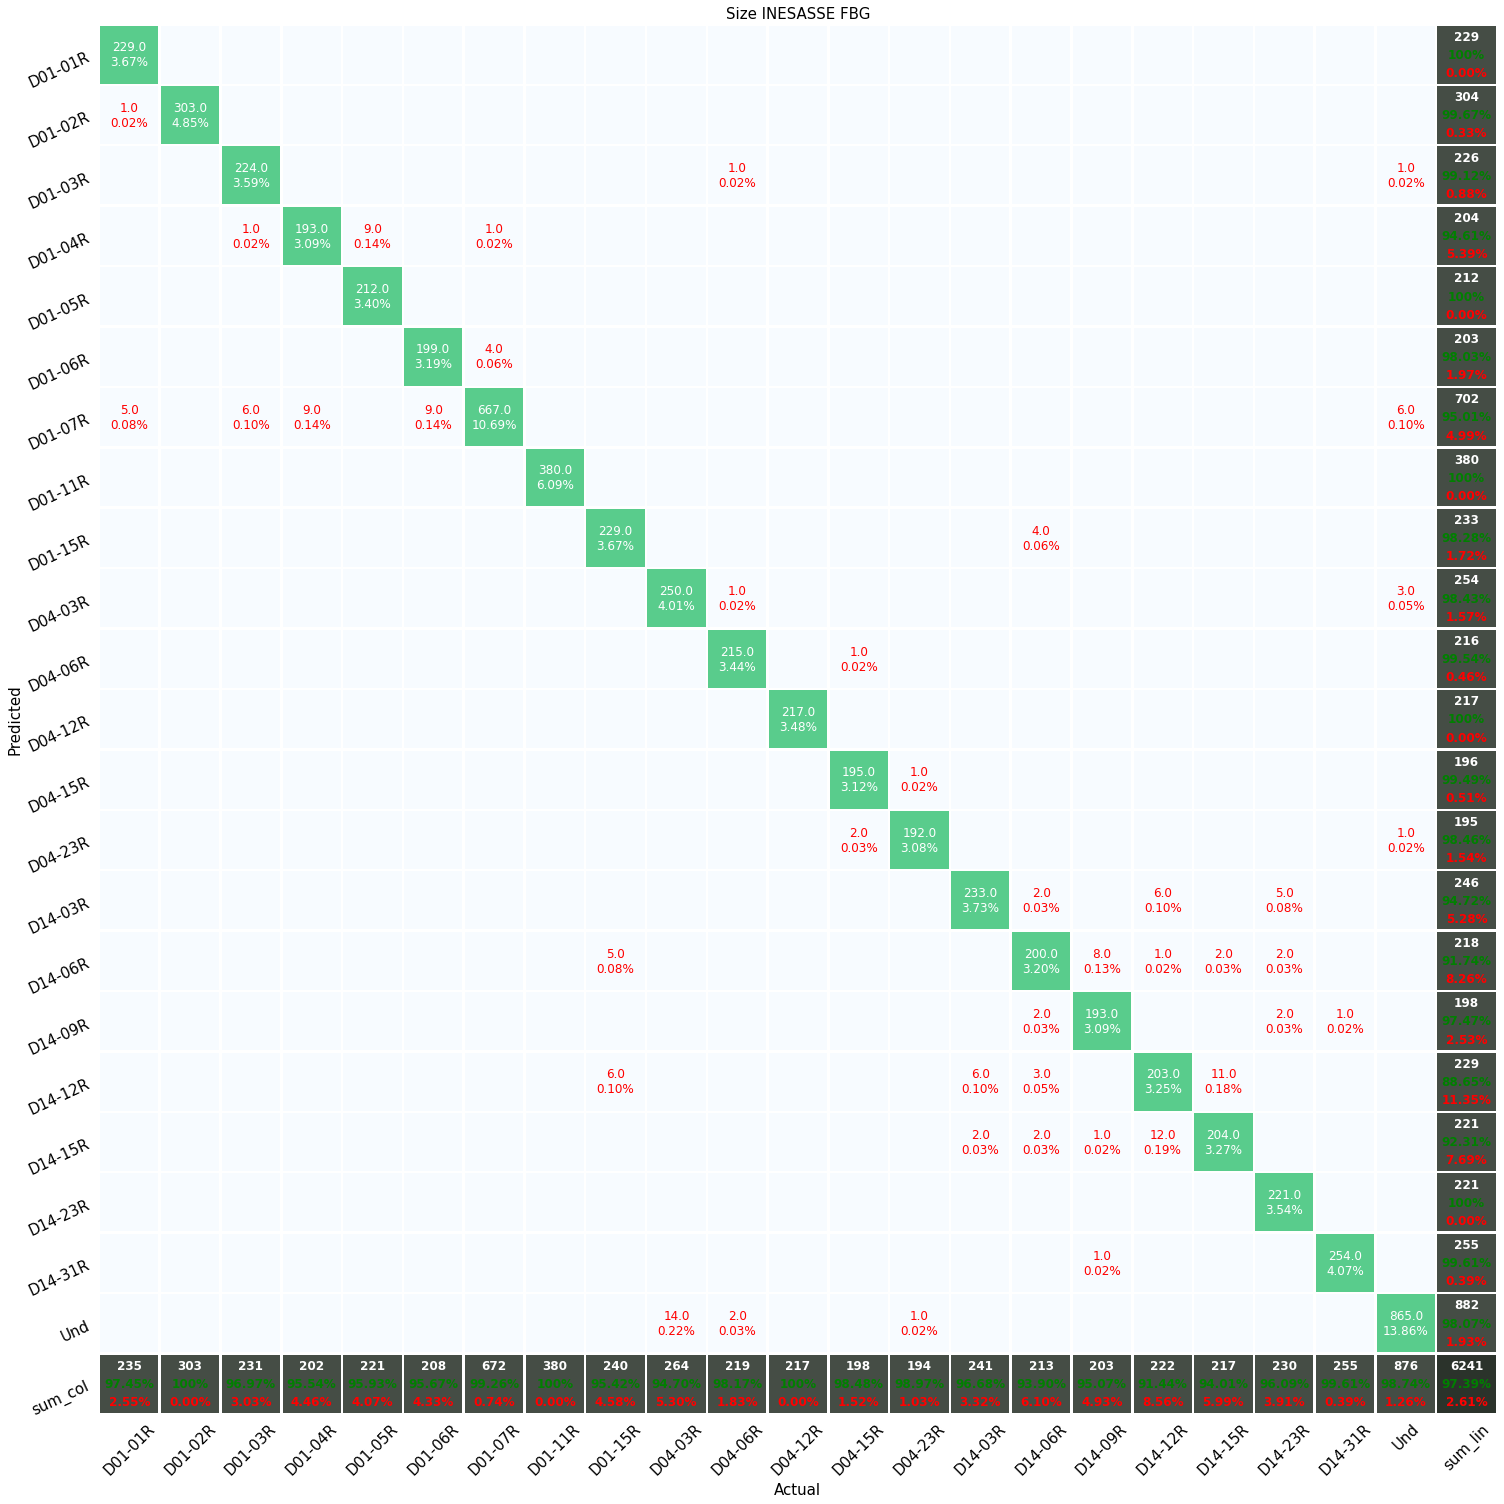
\includegraphics[width=125mm]{3/Fotos/Ty_Si_INESASSE_confusion.png}
        \captionsetup{justification=centering,margin=1.25cm}
        \caption{Matriz de confusión: Tamaños de daño}
        \label{fig:CM_FBG_Ty_Si}
    \end{figure} 

    \begin{figure}[H]
        \centering
        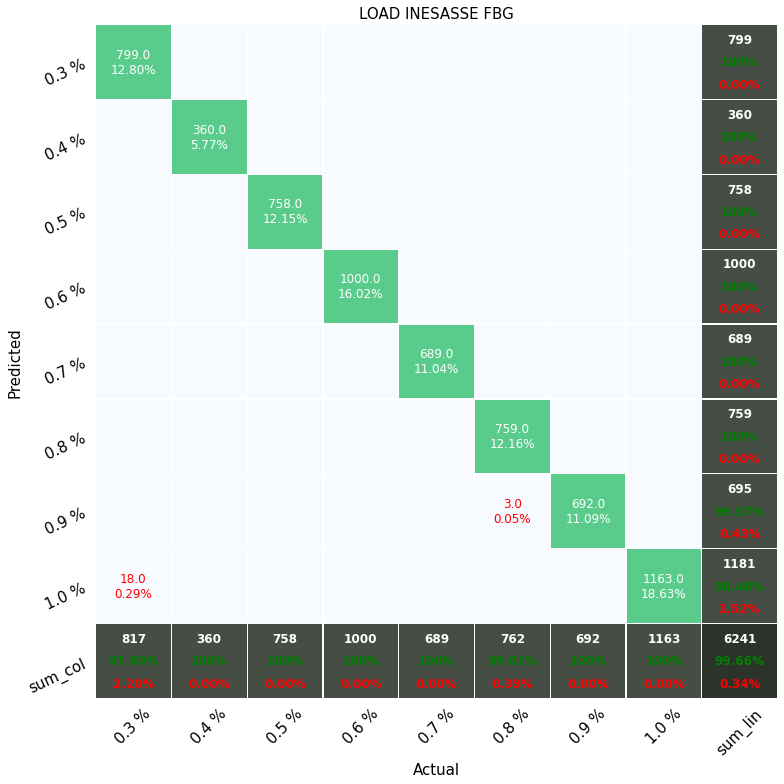
\includegraphics[width=125mm]{3/Fotos/Load_INESASSE_confusion.png}
        \captionsetup{justification=centering,margin=1.25cm}
        \caption{Matriz de confusión: Nivel de carga}
        \label{fig:CM_FBG_Load}
    \end{figure}  
  
    
	\item[$\bullet$] \textbf{Sensores OBR}    
    
    \begin{figure}[H]
        \centering
        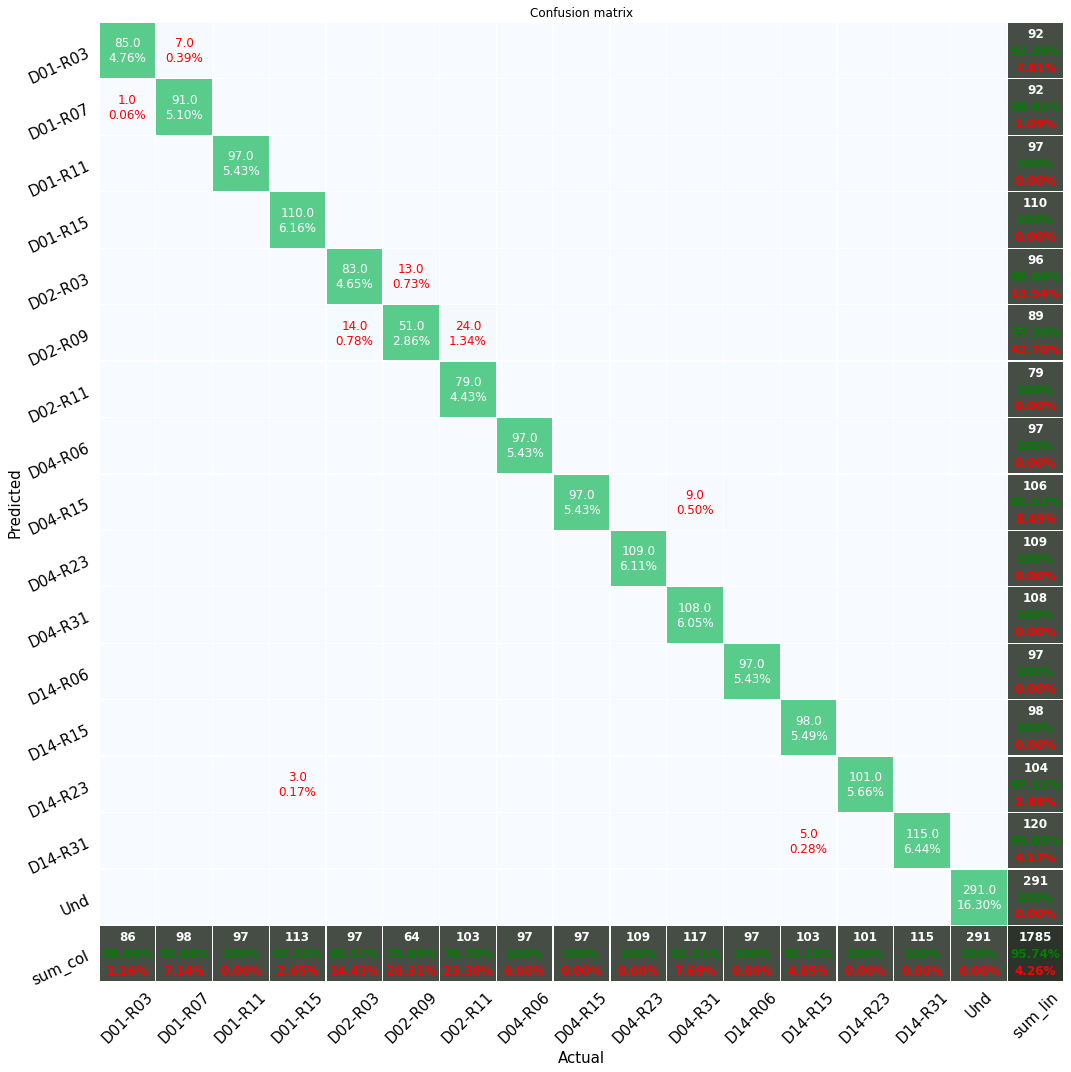
\includegraphics[width=125mm]{3/Fotos/CM_Ty_Si_OBR.png}
        \captionsetup{justification=centering,margin=1.25cm}
        \caption{Matriz de confusión: Tamaños de daño}
        \label{fig:CM_OBR_Ty_Si}
    \end{figure}  
    
    \begin{figure}[H]
        \centering
        \includegraphics[width=125mm]{3/Fotos/CM_Load_OBR.png}
        \captionsetup{justification=centering,margin=1.25cm}
        \caption{Matriz de confusión: Nivel de carga}
        \label{fig:CM_OBR_Load}
    \end{figure}      
    
    
\end{itemize}


%  -----------------------------------------  %


\clearpage

\section{Aplicación de DL al a la detección de cargas térmicas}

En una estructura aeronáutica no solo los daños provocan cambios en le campo de deformaciones, la temperatura también es un factor importante a tener en cuenta. Una aeronave puede estar sometida 50ºC en tierra y a -50ºC durante un vuelo. Este amplio rango de temperaturas genera cargas y deformaciones de un valor equivalente a las aerodinámicas.

Cuando la temperatura no es uniforme puede generar concentración de tensiones equivalentes a las que provoca un daño localizado, por lo que su estudio es apropiado en SHM.\\

Ya que este trabajo consiste en un una primera aproximación al uso de DL para la detección de cargas térmicas, solo se va a estudiar el caso de varias temperaturas uniformemente distribuidas.


% -- -- %


\subsection{Estructura bajo estudio}

Muchas de las estructuras aeronáuticas se pueden considerar vigas. Dependiendo de las cargas que vayan a soportar durante la operación, estas vigas estarán formados por unos componentes u otros.

\begin{figure}[h!]
 \centering
  \subfloat[Diagrama de una semiala]{
    \includegraphics[width=75mm]{3/Fotos/semiala_diagama.jpg}
    \label{fig:semiala}}
  \subfloat[Diagrama de un fuselaje]{
    \includegraphics[width=65mm]{3/Fotos/fuselage_diagam.png}
    \label{fig:fuselage}}
    \caption{Diagramas de estructuras aeronáuticas}
    \label{fig:estructuras}
\end{figure}

En la Figura \ref{fig:estructuras} se puede comparar una semiala con un fuselaje. Las semialas están sometidas a flexión y torsión, por ello estás formadas por larguerillos y costillas, sin embargo el fuselaje no trabaja a torsión, por lo que no tiene costillas.\\

Este estudio se ha centrado en la influencia de diferentes temperaturas sobre una viga con forma de omega y 4 costillas equiespaciadas, igual a la que se ve en la Figura \ref{fig:viga_real}. 

\begin{figure}[h!]
    \centering
    \includegraphics[width=100mm]{3/Fotos/Viga_Real.jpg}
    \captionsetup{justification=centering,margin=1.25cm}
    \caption{Imagen de la viga que se va a estudiar}
    \label{fig:viga_real}
\end{figure}     

Para obtener las deformaciones necesarias con las que se alimentará a la red se ha creado un modelo de elementos finitos (FEM). Las partes que forman el conjunto son los siguientes:
\begin{itemize}
    \item[$\bullet$] Tapa superior e inferior fabricada con laminado de 10mm
    \item[$\bullet$] Lateral izquiero y derecho fabricada con laminado de 4mm
    \item[$\bullet$] Costillas fabricadas con laminado de 4mm
\end{itemize}

Las características de los laminados se pueden ver en la Tabla \ref{tab:laminados}

\begin{table}[H]
    %\small
    \centering
    \begin{tabular}{|c|c|c|c|}
        \hline
        \textbf{Espesor laminado} & \textbf{Esperor capa} & \textbf{Número de capas} & \textbf{Orientación}\\ \hline
        10       & 0.2       & 50         & $[(\pm45, 90, 0, 90), 0_{15}]_{S}$  \\  \hline
        4        & 0.2       & 20         & $[(\pm45, 90, 0_{7}]_{S}$  \\\hline
    \end{tabular}
    \caption{Laminados} 
   \label{tab:laminados}
\end{table}

\begin{figure}[h!]
    \centering
    \includegraphics[width=150mm]{3/Fotos/L_BC.PNG}
    \captionsetup{justification=centering,margin=1.25cm}
    \caption{Viga con condiciones de contorno aplicadas}
    \label{fig:viga_bc}
\end{figure}     

En la Figura \ref{fig:viga_bc} se puede ver la viga ya en Patran después de haber creado las superficies y elementos y haber aplicado las condiciones de contorno. 

Las condiciones de contorno son las siguientes:

\begin{itemize}
    \item[$\bullet$] Carga vertical sobre distribuida sobre la parte superior de las costillas centrales
    \item[$\bullet$] Empotramiento de los nodos correspondientes a la parte inferior de los laterales.
\end{itemize}


% -- -- %


\subsection{Definición de daños y sensores}

En esta sección no solo se va a buscar clasificar la temperatura de una estructura, sino que también se le van a añadir dos tipos de daños típicos en estructuras de material compuesto.

Estos daños van van a ser los siguientes:
\begin{itemize}
    \item[$\bullet$] Despegue parcial de la tapa superior y uno de los laterales. Este daño se va a llamar D01
    \item[$\bullet$] Empotramiento de los nodos correspondientes a la parte inferior de los laterales.
\end{itemize}


Para obtener las deformaciones, se van a utilizar varias filas de elementos orientados en una misma dirección global. Con esto se consigue simular un sensor OBR similar al que se usó en el proyecto INESASSE. Se pueden ver los elementos que se han seleccionada para hacer de sensor OBR en la Figura \ref{fig:sensors}.

\begin{figure}[h!]
    \centering
    \includegraphics[width=150mm]{3/Fotos/Sensors.png}
    \captionsetup{justification=centering,margin=1.25cm}
    \caption{Tiras de sensores de los que se van a extraer las deformaciones}
    \label{fig:sensors}
\end{figure}  


% -- -- %










	
%------------------%


% \subsection{DACOMAT}

% \begin{itemize}
%     \item[$\bullet$] \textbf{CLASIFICACIÓN DE CARGA}
    
%     \begin{figure}[H]
%         \centering
%         \includegraphics[width=150mm]{3/Fotos/Load_DACOMAT_t-sne.png}
%         \captionsetup{justification=centering,margin=1.25cm}
%         \caption{Representación de los vectores de deformaciones tras reducir la dimensión de 400 a 2}
%         \label{def_h}
%     \end{figure}  
    
%     \begin{figure}[H]
%         \centering
%         \includegraphics[width=150mm]{3/Fotos/Load_DACOMAT_confusion.png}
%         \captionsetup{justification=centering,margin=1.25cm}
%         \caption{Matriz de confusión}
%         \label{def_h}
%     \end{figure}  
    
%     \item[$\bullet$] \textbf{CLASIFICACIÓN DE TEMPERATURA}
    
%     \begin{figure}[H]
%         \centering
%         \includegraphics[width=150mm]{3/Fotos/Temperature_DACOMAT_t-sne.png}
%         \captionsetup{justification=centering,margin=1.25cm}
%         \caption{Representación de los vectores de deformaciones tras reducir la dimensión de 400 a 2}
%         \label{def_h}
%     \end{figure}  
    
%     \begin{figure}[H]
%         \centering
%         \includegraphics[width=150mm]{3/Fotos/Temperature_DACOMAT_confusion.png}
%         \captionsetup{justification=centering,margin=1.25cm}
%         \caption{Matriz de confusión}
%         \label{def_h}
%     \end{figure}  
    
%     \item[$\bullet$] \textbf{CLASIFICACIÓN DE CASO DE DAÑO}
    
%     \begin{figure}[H]
%         \centering
%         \includegraphics[width=150mm]{3/Fotos/Ty_Si_DACOMAT_t-sne.png}
%         \captionsetup{justification=centering,margin=1.25cm}
%         \caption{Representación de los vectores de deformaciones tras reducir la dimensión de 400 a 2}
%         \label{def_h}
%     \end{figure}  
    
%     \begin{figure}[H]
%         \centering
%         \includegraphics[width=150mm]{3/Fotos/Ty_Si_DACOMAT_confusion.png}
%         \captionsetup{justification=centering,margin=1.25cm}
%         \caption{Matriz de confusión}
%         \label{def_h}
%     \end{figure} 
    
% \end{itemize}
 

	\clearpage
%	\clearemptydoublepage
    \chapter{Caracterización de impactos para SHM}

\section{ Propuesta de ensayo experimental }

    \subsection{Impactador estructura}

    \subsection{Electrónica - Software y hardware}

    \subsection{Adquisición y procesado de datos}

\clearpage

% -- -- %


\section{Caracterización de la posición}

CON DATOS DE CHRISTIAN Y AIRBUS AL MENOS

Red que clasifica la posición de un impacto

\clearpage

%  --  --  %


\section{Caracterización de la energía}

CON DATOS DE CHRISTIAN Y AIRBUS AL MENOS

Red que clasifica la energía de impacto.

\clearpage

%  --  --  %


\section{Caracterización de la velocidad}

Si se termina por realizar el impactador, también se buscará una clasificacion de velocidad da impacto para diferentes masas y misma altura de suelta.

\clearpage

%  --  --  %


\section{Caracterización completa de un impacto}

Combinación de los anteriores clasificadores para comprobar la precisión completa de un impacto.

\clearpage
    \clearpage
%	\clearemptydoublepage
    \chapter{Conclusiones y trabajos futuros}


\section{Conclusiones}

al menos 3-4 pags

\clearpage

%  --  --  %


\section{Trabajos futuros}

1 pag

    qewrg weqwewe  \cite{einstein}
    \clearpage
    
    
    
    %\bibliographystyle{apalike}
	\printbibliography %Prints bibliography
	\nocite{*}
    
\end{document}
